%\title{beavtex}
\documentclass[double,12pt]{beavtex}
\usepackage{graphicx}
\usepackage{lscape}
\usepackage{mathtools, nccmath}
\usepackage{array}
\usepackage{adjustbox}
\usepackage{rotating} %Package added to allow the rotation of figures and chart on a page, {sidewaysfigure} command
\usepackage{tablefootnote} %Packaged added to allow footnotes in the tabular environment, use \tablefootnote command
\usepackage[acronym]{glossaries}
\usepackage{nomencl}
\makenomenclature
\title{Validation and Verification Analysis for the OSU HTTF PG-28 Test}
\author{Joshua K Halsted}
\degree{Master of Science}
\doctype{Thesis}
\department{Nuclear Engineering and Radiation Health Physics}
\depttype{School}
\depthead{Director}
\major{Radiation Health Physics}
\advisor{Dr. Izabela Gutowska}
\submitdate{April 2, 2022}
\commencementyear{2022}



\makeglossaries

\newacronym{bc}{BC}{boundary condition}
\newacronym{cd}{CD}{cold duct}
\newacronym{cfd}{CFD}{computational fluid dynamics}
\newacronym{dpt}{DPT}{differential pressure transducers}
\newacronym{dns}{DNS}{director numerical solution}
\newacronym{eos}{EOS}{equation-of-state}
\newacronym{fvm}{FVM}{finite volume method}
\newacronym{ga}{GA}{General Atomics}
\newacronym{gci}{GCI}{gas concentration instrument}
\newacronym{hd}{HD}{hot duct}
\newacronym{htgr}{HTGR}{high temperature gas reactor}
\newacronym{httf}{HTTF}{High Temperature Test Facility}
\newacronym{iet}{IET}{integral effects test}
\newacronym{inl}{INL}{Idaho National Laboratory}
\newacronym{loca}{LOCA}{loss-of-coolant accident}
\newacronym{lp}{LP}{lower plenum}
\newacronym{mhtgr}{MHTGR}{modular high temperature gas reactor}
\newacronym{mfr}{MFR}{mass flow rate}
\newacronym{moose}{MOOSE}{Multiphysics Object Oriented Simulation Environment}
\newacronym{ns}{NS}{Navier-Stokes}
\newacronym{oandm}{O\&M}{operations and maintenance}
\newacronym{od}{OD}{outlet duct}
\newacronym{osu}{OSU}{Oregon State University}
\newacronym{pcs}{PCS}{primary coolant system}
\newacronym{pg}{PG}{Procedural Guide}
\newacronym{pirt}{PIRT}{Phenomena and Identification Ranking Table}
\newacronym{pt}{PT}{pressure transducers}
\newacronym{pwss}{PWSS}{potable water supply system}
\newacronym{r5}{R5}{RELAP5-3D}
\newacronym{r7}{R7}{RELAP7}
\newacronym{rans}{RANS}{Reynolds-Averaged Navier-Stoke}
\newacronym{rc}{RC}{reactor cavity}
\newacronym{rccs}{RCCS}{reactor cavity cooling system}
\newacronym{rcst}{RCST}{reactor cavity simulation tank}
\newacronym{rpv}{RPV}{reactor pressure vessel}
\newacronym{rsm}{RSM}{Reynolds stress model}
\newacronym{rx}{RX}{reactor core}
\newacronym{scs}{SCS}{secondary coolant system}
\newacronym{sg}{SG}{steam generator}
\newacronym{ss}{SS}{steady-state}
\newacronym{star}{STAR}{STAR-CCM+}
\newacronym{tc}{TC}{thermocouples}
\newacronym{tdj}{TDJ}{time dependent junction}
\newacronym{tdr}{TDR}{turbulent dissipation rate}
\newacronym{tdv}{TDV}{time dependent volume}
\newacronym{tf}{TF}{fluid temperature thermocouples}
\newacronym{tke}{TKE}{turbulent kinetic energy}
\newacronym{ts}{TS}{solid temperature thermocouples}
\newacronym{up}{UP}{upper plenum}
\newacronym{vandv}{V\&V}{validation and verification}


\makenomenclature
\nomenclature{$A$}{Cross-sectional area}
\nomenclature{$\alpha$}{Void fraction ($\alpha_{g}$ $\alpha_{f}$ are specific to gas and liquid, respectively)}
\nomenclature{$\epsilon$}{Turbulent dissipation rate for a unit mass (used for $k-\epsilon$ model)}
\nomenclature{$i$}{Fluid chemical thermal enthalpy}
\nomenclature{$\kappa$}{von Karman's constant)}
\nomenclature{$k$}{Turbulent kinetic energy (used for $k-\epsilon$ and $k-\omega$ model)}
\nomenclature{$\overrightarrow{f}_{b}$}{External body force exerted on fluid unit volume}
\nomenclature{$\overline{\overline{I}}$}{Identity matrix}
\nomenclature{$Ma$}{Mach number}
\nomenclature{$\nu$}{Kinematic viscosity}
\nomenclature{$\Tilde{nu}$}{Kinematic eddy viscosity parameter (used for Spalart-Allmaras model)}
\nomenclature{$\omega$}{Turbulent frequency, equal to $\epsilon/k$}
\nomenclature{$\phi$}{General transport scalar variable, equivalent to $\Phi + \phi^{'}$}
\nomenclature{$\phi^{'}$}{Fluctuating component of $\phi$}
\nomenclature{$\Phi$}{Mean component of $\phi$}
\nomenclature{$\rho$}{Fluid density}
\nomenclature{$\overline{\overline{\sigma}}$}{Stress tensor, equal to $-P \overline{\overline{I}} + \overline{\overline{T}}$}
\nomenclature{$\overrightarrow{v}$}{Velocity vector, equivalent to $u \hat{i} + v \hat{j} + w \hat{k}$}
\nomenclature{$P$}{Fluid pressure}
\nomenclature{$\overrightarrow{q}$}{Heat flux (into fluid)}
\nomenclature{$Q$}{Volumetric flow rate}
\nomenclature{$R$}{Specific gas constant}
\nomenclature{$R_{fluid}$}{Flow resistance}
\nomenclature{$Re$}{Reynolds number}
\nomenclature{$S_{E}$}{User-specified energy source term}
\nomenclature{$T$}{Fluid temperature}
\nomenclature{$\overline{\overline{T}}$}{Viscous stress tensor, equal to }
\nomenclature{$U_{\infty}$}{Free stream velocity}
\nomenclature{$u$}{x-component of $\overrightarrow{v}$}
\nomenclature{$u^{+}$}{Non-dimensional velocity}
\nomenclature{$v$}{y-component of $\overrightarrow{v}$}
\nomenclature{$w$}{z-component of $\overrightarrow{v}$}
\nomenclature{$y^{+}$}{Non-dimensional distance from wall}


\abstract{High temperature gas reactors (\acrshort{htgr}'s) have been  researched and operated commercially since the inception of the nuclear industry. Newer designs, such as the \acrlong{ga} (\acrshort{ga}) Modular \acrshort{htgr}, aim to lower capital costs by shifting towards smaller, more modular designs, although further cost reductions with respect to \acrlong{oandm} (\acrshort{oandm}) are needed to make this design more economical. One phenomena affecting \acrshort{oandm} is the thermal stratification that occurs within the \acrshort{htgr} \acrlong{lp} (\acrshort{lp}) as a result of differing fluid jet temperatures exiting the core. Powerful computational tools can be used to model this phenomena as a substitute for experiments, but must first be validated with experimental data. The \acrlong{osu} (\acrshort{osu}) \acrlong{httf} (\acrshort{httf}) \acrlong{pg} (\acrshort{pg}) 28 test was performed for this purpose, and this document details the effort to compare the experimental results with simulations performed at both the system and mesoscale levels.}


\acknowledgements{I would like to first thank my advisor, Dr. Izabela Gutowska, for the numerous opportunities afforded to me to work on scaled test facilities. This includes helping with the design of Kairos Power's SET facility in 2020 and writing reports pertaining OSU HTTF conduction cooldown tests and the SFSET in 2021. I would like to also thank Dr. Woods for his guidance with the HTTF and with Kairos while he was the principal investigator.

Next, I would like to thank INL scientists Dr. Paolo Balestra and Dr. Aaron Epiney for their assistance with the RELAP and MOOSE/Pronghorn models that I modified or created. Dr. Epiney helped me with understanding the HTTF RELAP deck and gave me starting points on automation scripts to use for modifying the base deck. Dr. Balestra was my mentor at INL during my summer internship, explaining the theory behind porous physics and how computer clusters worked. Both were patient and helpful in explaining concepts that I did not previously understand, and I am grateful. 

Graduate school was a period where I learned how to learn. It also taught me how to be patient and how to be resourceful and independent. I want to thank my mentors (Bill Walters, Mike Bingham and Randy Ellison), my supervisor (Keith Higar), and manager at the time Steve Lydzinski for helping reinforce these principles during my time at Framatome, and helping me learn a new way to program. This has opened up an entire new world for me, such that becoming a software engineer is where I want my career to go.

Special thanks to my fellow undergraduate and graduate students who I have sought help from, as well as assisted, when it came to both classwork and their specific projects. I have learned so much from these people not just about technical details of what we are studying, but also how to work in groups and build chemistry. The laughs and "aha!" moments were well worth the countless late nights. 

Last, I would like to thank my mom and dad for being supportive of my decision to pursue graduate school. It has opened up opportunities to work for employers that emphasize the value of good work and diligence. It was always a joy to come home and see you guys, as well as the 30+ animals on the property, and to remind myself to take time to enjoy things outside of my passion for engineering.}


\begin{document}
\maketitle
\mainmatter

%-------------------------INTRODUCTION-----------------------------

\chapter{Introduction}


\section{Background}

In its 2021 revision of the International Energy Outlook report \cite{eia_ieo}, the United States Energy Information Administration projects that world energy consumption will grow by nearly 50\% between 2020 and 2050 (see Figure \ref{fig:EIA_Projections}). Affordable energy production and distribution is vital for elevating and maintaining a high standard of living, and is a central reason why institutions around the world invest trillions of dollars into the energy sector annually \cite{iea_2021}.

\begin{figure}
    \begin{center}
    	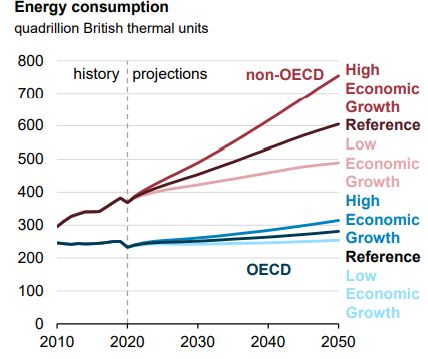
\includegraphics[width=10cm]{Figures/EIA_Projections.JPG}
    	\caption{World energy consumption projections (OECD and non-OECD)}
    	\label{fig:EIA_Projections}
    \end{center}
\end{figure}

Nuclear reactors are advertised as safe \cite{WN_Safety}, reliable \cite{mueller_2021}, and do not require as much land as other power production methods \cite{shellenberger_2021}. Reactors currently provide approximately 20\% of America's electricity needs, but only 4\% of global energy production \cite{eia_nuclear}. A central reason for why that share has not increased substantially since the technology's inception in the early 1950's is the economics associated with building, operating, and decommissioning \cite{touran}, as well as expanding into additional energy markets separate from electricity production \cite{process_heat}. One specific class of reactors that were designed to address these economic issues are \acrlong{mhtgr}s (\acrshort{mhtgr}s).  

\begin{figure}[!ht]
    \begin{center}
    	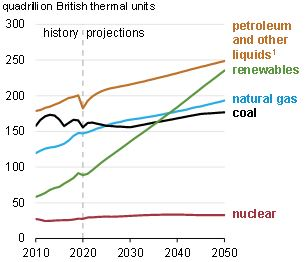
\includegraphics[width=8cm]{Figures/EIA_Projections_Sector.JPG}
    	\caption{Primary energy consumption by energy source (world)}
    	\label{fig:EIA_Projections_Sector}
    	\end{center}
\end{figure}

\begin{figure}[!ht]
    \begin{center}
    	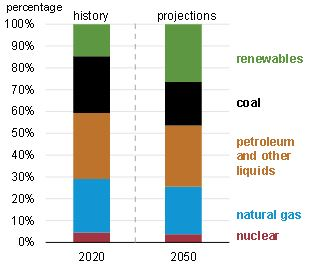
\includegraphics[width=8cm]{Figures/EIA_Projections_Source.JPG}
    	\caption{Share of primary energy consumption by source (world)}
    	\label{fig:EIA_Projections_Source}
    	\end{center}
\end{figure}

The \acrlong{ga} (\acrshort{ga}) \acrshort{mhtgr} \cite{murray} is similar to the design implemented at the Fort St. Vrains power plant in Colorado. It utilizes helium as the primary working fluid; ceramic, hexagonal prismatic blocks for both the fuel (TRISO kernels) and graphite reflector (see Figure \ref{fig:GA_MHTGR_Core_Block}); has fluid enter the \acrlong{rpv} (\acrshort{rpv}) via a concentric duct; and operates on a Brayton cycle (see Figure \ref{fig:GA_MHTGR_System} for basic operating characteristics). 

\begin{figure}[!ht]
    \begin{center}
    	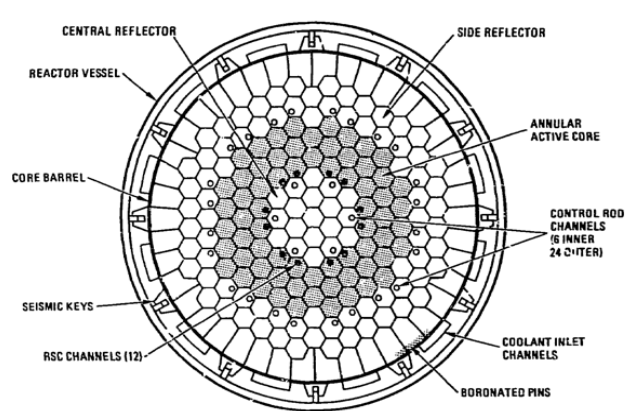
\includegraphics[width=10cm]{Figures/GA_MHTGR_Core_Block.PNG}
    	\caption{\acrshort{ga}-\acrshort{mhtgr} core block diagram}
    	\label{fig:GA_MHTGR_Core_Block}
    	\end{center}
\end{figure}

\begin{figure}[!ht]
    \begin{center}
    	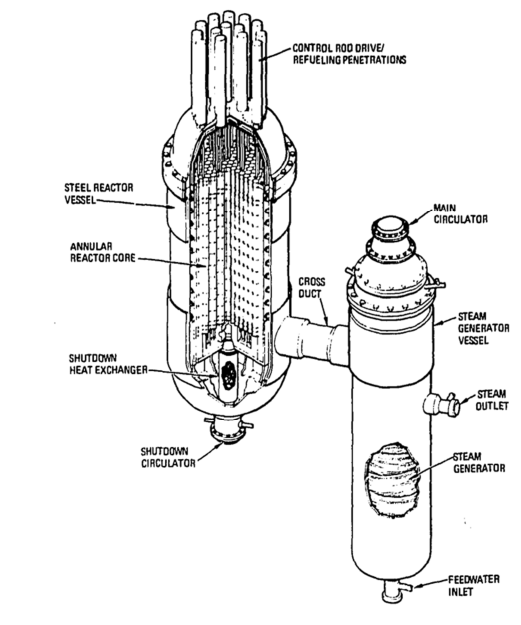
\includegraphics[width=8cm]{Figures/GA_MHTGR_System.PNG}
    	\caption{\acrshort{ga}-\acrshort{mhtgr} primary loop diagram}
    	\label{fig:GA_MHTGR_System}
    	\end{center}
\end{figure}

\begin{figure}[!ht]
    \begin{center}
    	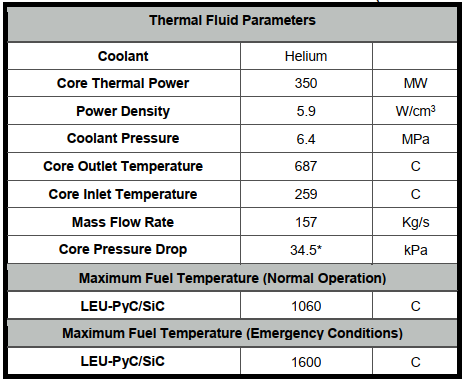
\includegraphics[width=10cm]{Figures/GA_MHTGR_Operating_Characteristics.PNG}
    	\caption{Some operating characteristics of the \acrshort{ga}-\acrshort{mhtgr}}
    	\label{fig:GA_MHTGR_Operating}
    	\end{center}
\end{figure}

In order to complete the licensing of such a design, phenomena unique to the reactor design (see \acrlong{pirt}, or \acrshort{pirt} \cite{ball_2008}) must be properly characterized, particularly with the use of computer codes. Important phenomena specific to normal operations include:
\begin{itemize}
    \item Understanding the flow distribution in the \acrshort{lp};
    \item Characterizing the bypass flow through the core; and
    \item Generating power and flux profiles.
\end{itemize}
All three are ranked with high importance, and low or medium knowledge. The first phenomena is particularly important because the \acrshort{lp} is where the helium coolant is the hottest, but because the fluid jets exiting the core have different temperatures, the \acrshort{lp} material may experience significant temperature gradients \cite{osti_1038194}. This may cause large internal stresses and result in the material cracking. Understanding the range of temperatures that may exist in these jets is the first step in alleviating thermal stresses and potentially lowering \acrshort{oandm} costs.


These codes, if validated with experimental data, can be used to simulate a spectrum of operating scenarios to prove that the reactor is indeed safe to operate. Part of this validation process incorporates using scaled \acrlong{iet} (\acrshort{iet}) facilities to gather experimental data, which is compared to computational results from system level codes and \acrlong{cfd} (\acrshort{cfd}) solvers. These \acrshort{iet}'s are particularly useful since they are less expensive and easier to manage than a full-scale prototype. One such facility is the \acrshort{osu} \acrshort{httf} (see Figure \ref{fig:HTTF_Shell} for facility rendering). From 2015 to 2019, the \acrshort{osu} \acrshort{httf} was used to collect data for tests performed intended to simulate basic shakedown and heat-up tests, conduction cooldown events, and normal operations. 

\begin{figure}
    \begin{center}
    	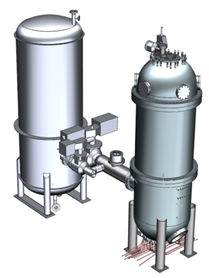
\includegraphics[width=8cm]{Figures/HTTF_Shell}
    	\caption{3D rendering of the \acrshort{httf}.}
    	\label{fig:HTTF_Shell}
    	\end{center}
\end{figure}

\section{Objective}

The objective of this thesis is to utilize computational methods and experimental data for one of the normal operations tests in order to perform a \acrlong{vandv} (\acrshort{vandv}) analysis at both the system level and in the \acrshort{lp}/\acrlong{od} (\acrshort{od}) region. The quantitative results (and qualitative reasons for the results) from this effort will provide the reader a general idea of how well both a systems-level and a \acrlong{fvm} (\acrshort{fvm}) solver actually simulate a normal operations scenario in the \acrshort{osu} \acrshort{httf}. From this, suggestions for improvement and a recommendation for using the two pieces of software to simulate future similar tests will be provided.


%------------------------LIT REVIEW--------------------------------

\chapter{Literature Review}

The first part of this literature review explains different aspects of the \acrshort{httf}, specifically the facility layout, instrumentation, and the  \acrlong{pg} 28 LP mixing test (\acrshort{pg}-28). The second part discusses the nature of system codes, and how they are used to model phenomena in large facilities. The third part discusses \acrshort{fvm} solvers, and why they are applicable to the complicated flow region that is the \acrshort{httf} \acrshort{lp}. The fourth and final section explains the process of validation and verification. 

\section{\acrshort{httf} – Facility Description and Experiments}

To summarize \cite{woods}, the facility contains the \acrlong{pcs} (\acrshort{pcs}) which has an \acrshort{rpv}, a concentric pipe consisting of the hot and cold ducts (\acrshort{hd} and \acrshort{cd}), a \acrlong{sg} (\acrshort{sg}), a gas circulator (GC), and connecting pipes. Break valves in both the hot and cold legs connect to a \acrlong{rcst} (\acrshort{rcst}); by which the gas composition can be manipulated to simulate the various thermodynamic conditions that may exist outside of the RPV following a \acrlong{loca} (\acrshort{loca}). The \acrshort{rpv} is surrounded by the \acrlong{rccs} (\acrshort{rccs}), which consists of cooling panels. Water flows upwards across the panels in order to cool the \acrshort{rpv} (water is supplied by the same tank that provides water to the \acrshort{sg}); this implies that the temperature of the \acrshort{rpv} can be controlled via altering the \acrlong{mfr} (\acrshort{mfr}) of water. Isolation valves can close off the supply of water in order to simulate a compromised heat sink. 

\begin{figure}
    \begin{center}
    	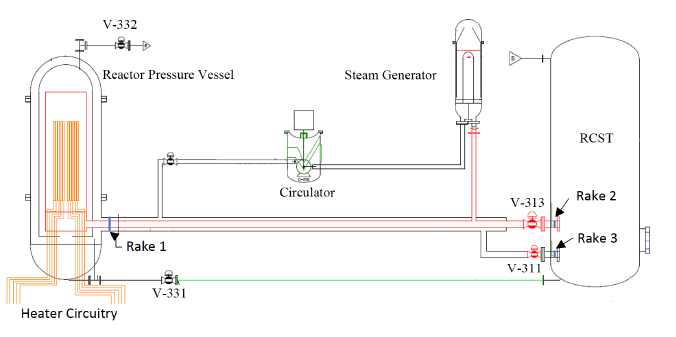
\includegraphics[width=12cm]{Figures/HTTF_Simple_Facility_Diagram.png}
    	\caption{Simplified system diagram of the \acrshort{httf} \cite{brumback_2020}.}
    	\label{fig:HTTF_Facility_Schematic}
    	\end{center}
\end{figure}

This section is to describe the layout, instrumentation, and tests related to the \acrshort{httf} with respect to the most relevant sections of the facility, which is the \acrlong{rx} (\acrshort{rx}), lower plenum (LP), and \acrshort{hd}. Although part of the scope of this report is to outline V\&V of data from two tests performed on the \acrshort{httf} (which looks at all thermophysical data generated from the entire facility), particular details is given to geometries inside the \acrshort{httf} that are most important to lower plenum mixing. 

\subsection{\acrshort{rx} and \acrshort{lp} Layout}

Figure \ref{fig:HTTF_RPV_Cutaway} shows a cross section of a 3D rendering of the \acrshort{httf} \acrshort{rpv}. Within the \acrshort{rpv} is the \acrshort{rx}. The \acrshort{rx} consists of an \acrlong{up} (\acrshort{up}), which is essentially an empty cavity. Below the \acrshort{up} are a series of stacked alumina ceramic blocks, which simulate both the core and the upper/lower reflectors of the GA MHTGR. Surrounding these blocks are ceramic blocks that represent the side reflector. Underneath these ceramic blocks is a roof, which covers the LP chamber and the LP floor/supports. All components in the RX are composed of Greencast-94F Plus  in order to withstand the high temperatures. See Figure \ref{fig:HTTF_Core_Blocks} for a diagram of the \acrshort{httf} \acrshort{rx}. Cold gas enters the core through the CD (which is the outer portion of the concentric pipe entering the \acrshort{rpv}), flows upwards through the \acrshort{rpv} between the side reflector blocks and the core barrel. Gas mixes in the \acrshort{up}, then flows down through the ceramic blocks via coolant channels.

\begin{figure}
    \begin{center}
    	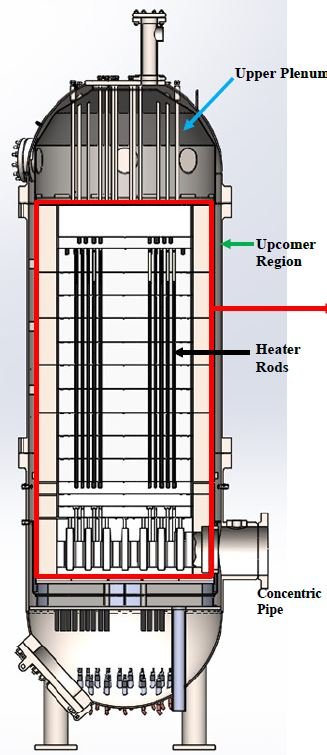
\includegraphics[width=5cm]{Figures/HTTF_RPV_Cross_Section.JPG}
    	\caption{\acrshort{httf} \acrshort{rpv} cutout}
    	\label{fig:HTTF_RPV_Cutaway}
    	\end{center}
\end{figure}

\begin{figure}
    \begin{center}
    	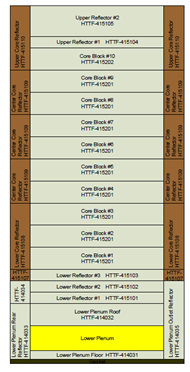
\includegraphics[width=5cm]{Figures/HTTF_Core_Blocks}
    	\caption{\acrshort{httf} \acrshort{rx} Layout.}
    	\label{fig:HTTF_Core_Blocks}
    	\end{center}
\end{figure}

The helium coolant flows through the \acrshort{lp} roof and impinges on the \acrshort{lp} floor (see Figure \ref{fig:LP_Velocity_Streamlines} for a computational representation). Between the roof and the floor is a chamber by which jets of coolant can mix prior to exiting. The coolant than exits at a nearly 90 degree bend through the \acrshort{hd}. The \acrshort{hd} is a pipe which connects to the \acrshort{sg}.

\begin{figure}
    \begin{center}
    	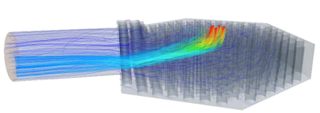
\includegraphics[width=10cm]{Figures/LP_Velocity_Streamlines}
    	\caption{Visualization of how helium coolant passes through \acrshort{httf} \acrshort{lp}.}
    	\label{fig:LP_Velocity_Streamlines}
    	\end{center}
\end{figure}

\subsection{\acrshort{httf} Instrumentation}

\subsubsection{Summary}

The \acrshort{httf} has 400 data acquisition channels including \acrshort{tc}'s, \acrlong{pt}s (\acrshort{pt}'s), \acrlong{dpt}s (\acrshort{dpt}'s), flow meters, and gas sensors. In total, the entire \acrshort{httf} has over 500 instruments. Since the scope of this document pertains both to \acrshort{vandv} of the \acrshort{httf}, as well as examining mixing phenomena in the LP, the following subsections have been written to detail what type of instruments were used in both LP mixing experiments, with emphasis on the \acrshort{lp} and the \acrshort{od}. A brief description of the instruments used in other parts of the \acrshort{httf} is also provided. Consult the \acrshort{osu} \acrshort{httf} Plan \cite{louria} for further details.

\subsection{Lower Plenum}

The \acrshort{lp} consists of multiple types of \acrshort{tc}'s, pressure sensors (taps), and g\acrlong{gci} (\acrshort{gci}’s). In order to support these instruments, a total of 163 ceramic support posts were implemented into the \acrshort{lp} floor. 16 of these can support \acrshort{tc}'s. These support posts are spaced (Figure \ref{fig:HTTF_LP_Support_Posts}) such that they create “jets” of hot air, which are then routed through the side of the support posts via 0.6 cm diameter channels at 25\% and 75\% of the support posts (\acrshort{lp} height). 

\begin{figure}
    \begin{center}
    	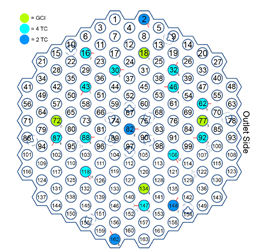
\includegraphics[width=10cm]{Figures/HTTF_LP_Support_Posts.png}
    	\caption{Diagram showing \acrshort{tc}'s and gas detectors in the LP. Channels with 4 \acrshort{tc}'s have \acrshort{tc}'s located at the gas inlet, upper, lower, and floor, while those with only 2 are located at the upper and lower.}
    	\label{fig:HTTF_LP_Support_Posts}
    	\end{center}
\end{figure}

There are 58 K-type \acrshort{tc}'s that are used within the \acrshort{lp}. 32 are gas \acrshort{tc}'s, 12 are gas \acrshort{tc}'s installed at the LP inlet, 12 are ceramic material \acrshort{tc}'s installed into the \acrshort{lp} floor, and 2 are ceramic material \acrshort{tc}'s installed into the side reflector of the \acrshort{lp} to measure solid material temperatures. See Figure \ref{fig:HTTF_LP_PT_Placement_Axial} for an elevation layout for two support columns that are aligned specifically to both measure temperatures for gas jets and air ingress. A radial layout of the \acrshort{tc}'s in the \acrshort{lp} is provided in Figure \ref{fig:HTTF_LP_PT_Placement_Radial}.

\begin{figure}
    \begin{center}
    	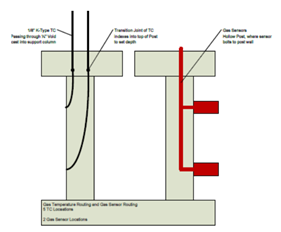
\includegraphics[width=8cm]{Figures/HTTF_LP_PT_Placement_Axial.png}
    	\caption{Elevation layout for \acrshort{tc}'s in two adjacent support columns used for jet characterization. The black circles represent \acrshort{tc}'s used for measure temperatures in the inlet plenum, 25\% \acrshort{lp} height, and 75\% \acrshort{lp} height. The purple circle represents a single \acrshort{tc} used for measuring solid material temperature of the \acrshort{lp} floor..}
    	\label{fig:HTTF_LP_PT_Placement_Axial}
    	\end{center}
\end{figure}

\begin{figure}
    \begin{center}
    	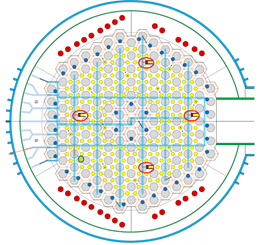
\includegraphics[width=10cm]{Figures/HTTF_LP_PT_Placement_Radial.png}
    	\caption{\acrshort{tc} Locations within the \acrshort{lp}. Purple circles represent \acrshort{tc}'s used to measure side reflector temperatures; black represents \acrshort{tc}'s used to measure gas temperatures at 25\% and 75\% of the \acrshort{lp} height; blue circles represent 4 \acrshort{tc}'s used for jet characterization and \acrshort{lp} floor temperatures}
    	\label{fig:HTTF_LP_PT_Placement_Radial}
    	\end{center}
\end{figure}

One pressure tap is located near the edge of the \acrshort{lp} opposite the side containing the inlet and outlet ducts. This pressure tap is connected to a \acrshort{dpt}; the reference pressure for this \acrshort{dpt} is the \acrshort{rpv} inlet pressure. Within four of the support columns previously described, there are gas sensors located at both the 25\% and 75\% of the \acrshort{lp} height, and are located on the opposite side of the \acrshort{tc}'s.  

\subsection{Outlet Duct and Hot Leg}

The Outlet Duct (also known as the Hot Leg) consists of K-type \acrshort{tc}'s, plate-type \acrshort{gci}'s, and pressure sensor instrumentation. These instruments are encapsulated into a “rake” (see Figure \ref{fig:Rake_Figure}). Three rakes are located either at the entrance of the \acrshort{rpv}, or downstream of it. Rakes 1 and 2 penetrated into the outlet duct. Within each rake, \acrshort{tc} and \acrshort{gci}’s are “stacked” vertically (see Figure \ref{fig:HTTF_HD_Rake_TCs}). The \acrshort{gci}’s are placed on a pair of red airfoils; each airfoil consists of two \acrshort{gci} plates, situated at the same elevation, in order to provide a capacitive reading on the gas concentrations.  Rake 1 also consists of pressure taps at the top of the Hot Leg and Cold Leg; a static pressure sensor is located at the top of the Cold Leg pressure tap to provide a baseline system pressure. This pressure provides the reference pressured used in the \acrshort{dpt}'s for the primary system.

\begin{figure}
    \begin{center}
    	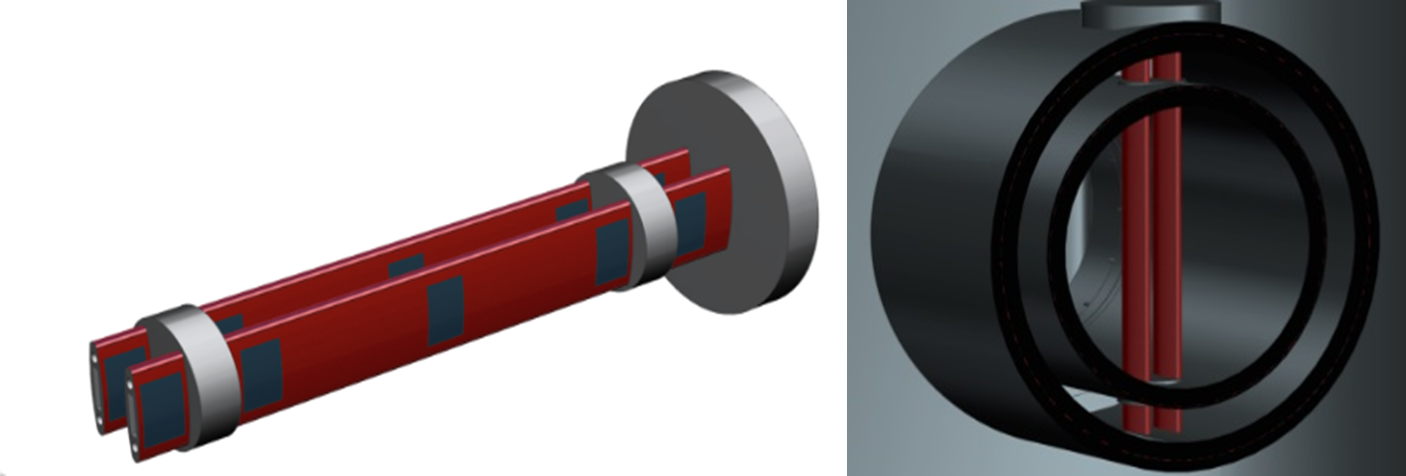
\includegraphics[width=8cm]{Figures/Rake_Figure.png}
    	\caption{CAD model of the rake containing \acrshort{tc}'s and \acrshort{gci}'s}
    	\label{fig:Rake_Figure}
    	\end{center}
\end{figure}

\begin{figure}
    \begin{center}
    	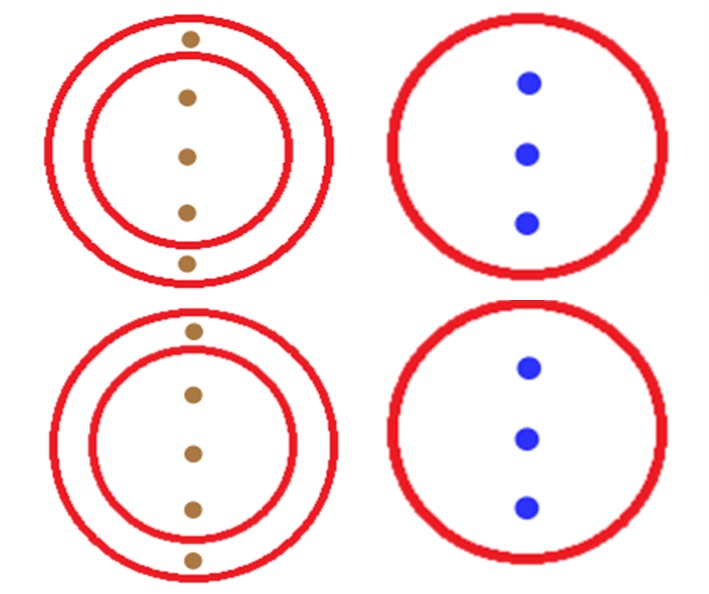
\includegraphics[width=7cm]{Figures/HTTF_HD_Rake_TCs.png}
    	\caption{Locations of instruments within Hot Legs (inner) and Cold Legs (outer). top left is the TC layout in Rake 1; top right is the \acrshort{tc} layout in Rake 2; bottom pictures are the \acrshort{gci} layouts in Rakes 1 and 2}
    	\label{fig:HTTF_HD_Rake_TCs}
    	\end{center}
\end{figure}


\section{\acrshort{pg}-28 Test Description}

This section details the test conducted in order to examine phenomena in the \acrshort{httf} \acrshort{lp} region. The \acrshort{pg}-28 test was conducted in order to examine thermal profiles and mixing phenomena in the LP due to changes in the system \acrshort{mfr}. The power to the heaters was constant (see Figure ...). The primary system \acrshort{mfr} was increased three times, leading to jumps in heat removal rates in the core, resulting in temporary higher coolant temperatures in the \acrshort{lp} (see Figure 13). The core was heated up over 47 hours until a hot \acrlong{ss} (\acrshort{ss}) was reached, which incorporated that the:

\begin{itemize}
    \item Peak core temperature is between 780 and 820$^{o}$ C;
    \item Core average temperature is between 525 and 575$^{o}$ C; and
    \item No channel temperature increases greater than 5$^{o}$ C per hour;
\end{itemize}

Additional conditions that had to be met are outlined in Figure \ref{fig:PG_28_Initial_Conditions}. Core temperatures were allowed to increase throughout the core, so long as material requirements were not exceeded and heater power was relatively steady. As these core temperatures increased, the water level in the \acrshort{sg} decreased. Once it decreased below 60\%, the \acrshort{sg} inlet valve was opened to increase the water level. The \acrshort{rccs} was continuously operated with a motor speed of 30\%. The entire test last around 6.5 hours.

\begin{figure}
    \begin{center}
    	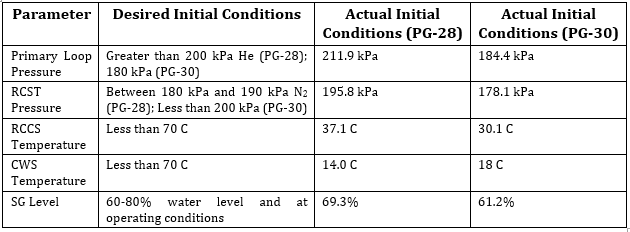
\includegraphics[width=10cm]{Figures/PG_28_Initial_Conditions.PNG}
    	\caption{Initial conditions for the \acrshort{pg}-28 test}
    	\label{fig:PG_28_Initial_Conditions}
    	\end{center}
\end{figure}

\section{System-Level Codes}

Traditionally, evaluating the performance of nuclear power plants during accident conditions has been achieved using system thermal hydraulic codes. Original system codes were developed according to conservative model assumptions; however, operators asked for codes that performed “best estimate” analysis, which simulated accidents as realistically as possible. Best-estimate thermal-hydraulic codes (e.g. RELAP, TRAC, CATHARE, ATHLET) are generally based on two-phase flow equations resolved in Eulerian coordinates. The two-phase flow field is described by mass, momentum, and energy conservation equations for the liquid and vapor phases separately and mass conservation equations for noncondensable gas present in the mixture. Originally, these codes modelled the entire systems in 1D, but later development allowed for components to be modelled in 3D. Such codes typically do not permit turbulent (eddy) modelling; thus, they are best applied to general piping systems or to systems that are large enough such that the general bulk flow behavior is not whirling.

As previously mentioned, these codes can be used in conjunction with \acrshort{cfd}  codes in order to model whole systems, and performing detailed analysis for a small region, such as a reactor core or a plenum. This is because system codes can model (transient) bulk fluid phenomena very quickly using either a fully-, semi-, or nearly-implicit scheme. Whereas for light water reactor modelling, where two sets of equations are needed to model both water and vapor, only one set of conservation equations is needed in order to model gas coolant, such as helium in the \acrshort{httf} . This should speed up code performance significantly when simulating testing conditions. 

\subsection{RELAP5-3D}

\acrshort{r5} is the latest code version of a series of codes developed by Idaho National Lab [11], originally developed to model accidents and operational transients in light-water reactor systems. It has the capability to simulate a wide variety of hydraulic and thermal transient behavior for both nuclear and non-nuclear systems. In addition to solving continuum equations (and having built in equations of state), the code had neutronic kinetics modeling capability. Turbomachinery such as pumps, valves, compressors, accumulators, etc. are available within the code.  

\subsubsection{Code Architecture}

\acrshort{r5} is coded with a top-down structuring that utilizes modularity. Each model and procedure is isolated into separate subroutines (subroutines are essentially functions that don’t return output). The top-most structure consists of input (INPUTD), transient/\acrshort{ss} (TRNCTL), and stripping (STRIP) blocks. The first and third blocks are relatively simple; INPUTD consists of three main processing phases:

\begin{itemize}
    \item Read input data, check for syntax errors, store data;
    \item Restart data is read, and input data is processed again;
    \item Cross-checking interrelationships of various types of data, and cross-linking of data blocks is completed.
\end{itemize}

STRIP extracts simulation data from a plot file to facilitate information exchange between \acrshort{r5} and other programs (such as Excel). 

The TRNCTL block handles both transient and \acrshort{ss} options. Both options are relatively similar in functionality; however, the \acrshort{ss} option only works if the program determines that \acrshort{ss} conditions are met (this occurs when if convergence testing algorithms conclude that \acrshort{ss} is reached). Often, a problem will be ran in transient mode from an initial state until time derivatives for certain thermophysical properties approach zero. 

Figure \ref{fig:RELAP_Block_Structure} details the structure of the TRNCTL block structure. Subroutine TRNSET essentially sets up the infrastructure needed in order to manage the output of such an analysis (cross-linking data block information, creates arrays for solution control, manages memory). TRAN controls the transient advancement of the solution. TRNFIN releases computational space for data blocks no longer needed, once TRAN has executed.

\begin{figure}
    \begin{center}
    	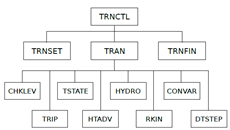
\includegraphics[width=10cm]{Figures/RELAP_Block_Structure.png}
    	\caption{Transient/\acrshort{ss} block structure for \acrshort{r5}  [need reference]}
    	\label{fig:RELAP_Block_Structure}
    	\end{center}
\end{figure}

To provide a brief summary about the TRAN block, CHKLEV controls two-phase mixture levels between volumes (volumes are defined in the input deck). TRIP evaluates logical statements that result in true or false statements (e.g. trip values can open or close valves). TSTATE provides fluid thermodynamic state information, and computes velocities for time-dependent junctions. HTADV calculates the heat transferred across solid boundaries of hydrodynamic volumes. HYDRO advances the hydrodynamic solution. In \acrshort{r5}, there is an option to model reactor kinetics with the RKIN subroutine; this subroutine uses the NESTLE code to compute power. Control systems used in hydrodynamic systems can be simulated with CONVAR. Last, DTSTEP determines the temporal step size and whether transient advancements should be terminated. With respect to the input model for the \acrshort{httf} (elaborated more in the next section), all but the RKIN modules are utilized.

\subsubsection{Hydrodynamic Model}

\acrshort{r5}’s hydrodynamic models is a transient, two-fluid model for flow of a two-phase vapor/gas-liquid mixture that has to capability to contain noncondensable components, soluble components, and radionuclides. It solves eight field equations for eight primary dependent variables. In the event that reactor kinetics are not being taken into account, and noncondensables do not exist within the two-phase flow, the number of equations reduces to six. These equations and dependent variables are listed in Table 4 along with variable nomenclature and meaning. These equations can be expanded to incorporate either 1D, 2D, or 3D geometries. The independent variables for these equations are time and space, which can be defined either in Cartesian or cylindrical coordinates.

\acrshort{r5}’s hydrodynamic spatial domain is split up spatially into volumes (for 3D analyses) and junctions. Volumes are essentially stream tubes that have an inlet and outlet. Every volume in \acrshort{r5} has an associated length, volume, flow area, vertical angle, wall roughness, hydraulic diameter, flags (boron presence, type of fluid present), and initial conditions. Positive vertical elevation defines a volume if the fluid flows from a lower elevation to a higher one. A volume can be used to impose pressure or temperature \acrlong{bc}s (\acrshort{bc}'s) (these are called \acrlong{tdv}s (\acrshort{tdv}’s). Junctions are entities that join volumes together. Each junction has flags, a flow area, initial conditions, and information about what volumes are upstream and downstream of the junction. Just like \acrshort{tdv}’s, junctions can be used to impose \acrshort{bc}'s such as velocity or \acrlong{mfr} (\acrshort{mfr}) in a time-dependent manner. These are called \acrlong{tdj}s (\acrshort{tdj}’s) and can be used to model flow components such as valve. \acrshort{tdv}’s and \acrshort{tdj}’s are used extensively when coupling \acrshort{r5}  with \acrshort{cfd}  codes. 

The discretization of the hydrodynamic model for \acrshort{r5} is based on a “room and doors” concept, which is a upwind-difference scheme based staggered spatial mesh where scalar properties are defined in “rooms” and vector quantities at “doors”. The net accumulation of mass and energy in a volume is the difference between what enters (plus sources) and what exits. This is then averaged over the entire volume and “set” at the volume’s center (the “room”). At this point (the center of the volume), there must be an associated velocity (momentum flux) associated with this mass and energy. This velocity defines a “door”. See Figure \ref{fig:RELAP_Room_Doors} for a visualization of the rooms and doors concept.

\begin{figure}
    \begin{center}
    	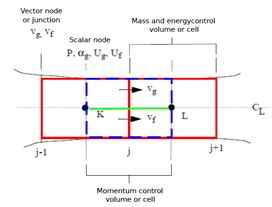
\includegraphics[width=10cm]{Figures/RELAP_Room_Doors.png}
    	\caption{\acrshort{r5} rooms and doors concept, also known as a staggered grid approach}
    	\label{fig:RELAP_Room_Doors}
    	\end{center}
\end{figure}

The code is solved numerically using a semi-implicit finite-difference technique by default (typically used for transients), or, if specified by the user, a nearly-implicit finite-difference technique, which allows violation of the material Courant limit (ideal for slowly varying transient calculations). This scheme is first order accurate in both space and time. The nature of the two-fluid differential equations constitute an ill-posed initial boundary value problem, but the introduction of artificial terms enable the problem to be well-posed. Reynolds stress-like terms, which are necessary for modelling eddying flows, are not incorporated into the numerical scheme. Time step advancement is manipulated by the code in order to ensure a stable solution; the code utilizes a direct lower-upper factorization scheme in order to solve the linearized system of conservation equations. Overall, \acrshort{r5} has been to be consistent, stable, and convergent for the two-fluid model.

\subsubsection{Heat Structure Model}

Calculations of heat transfer across the solid boundaries of hydrodynamic volumes are performed through “heat structures”. These structures are typically rectangular, cylindrical, or spherical; this inclusion of a radial dimension gives it more capability for modelling compared to the hydrodynamic components. Similar to the hydrodynamic module, a finite-difference method (specifically, Crank-Nicolson) is used to solve the heat transfer equation; specifically, . This method is unconditionally stable and second-order accurate with respect to time. The \acrshort{bc}'ss that can be implemented for these heat structures include allowing symmetry or insulating conditions, custom heat transfer correlations, and time-dependent quantities such as heat flux and power.

\subsubsection{\acrshort{r5} Input Model for \acrshort{httf}}

Original development of a \acrshort{r5} input model for the \acrshort{httf} was developed by \acrshort{inl} and Bayless [12] to resemble the \acrshort{ga} \acrshort{mhtgr} as closely as possible mainly by scaling the reference height and radial dimensions by a quarter, in order to obtain rough estimates for natural circulation scaling factors. This model includes the \acrshort{rpv}, reactor cavity atmosphere, and RCCS. Bayless and \acrshort{inl} later revised this model to more accurately the geometry of the \acrshort{httf} according to the 2018 version drawings and layout document. This updated version consists of modelling the alternate break piping, \acrshort{rpv}, \acrshort{pcs}, \acrlong{scs} (\acrshort{scs}), \acrlong{pwss} (\acrshort{pwss}), \acrlong{rc} (\acrshort{rc}), and (\acrshort{rccs}). The model includes hydrodynamic components, heat structures, trips, and control systems. With respect to the hydrodynamic modelling, the numbering scheme goes as follows:
\begin{itemize}
    \item 1-99: alternate break piping (not used for any tests);
    \item 100-199: \acrshort{rpv};
    \item 200-299: \acrshort{pcs} piping/components;
    \item 300-399: \acrshort{scs} piping/components;
    \item 400-499: \acrshort{pwss}
    \item 900-999: \acrshort{rc} and \acrshort{rccs}
\end{itemize}

See Figure \ref{fig:HTTF_RELAP_Nodalization} for the general \acrshort{httf} nodalization diagram. A brief description of the nodalization techniques used to model the hydrodynamic components needed for the input deck of the \acrshort{rpv} is provided in the next section. 

\begin{figure}
    \begin{center}
    	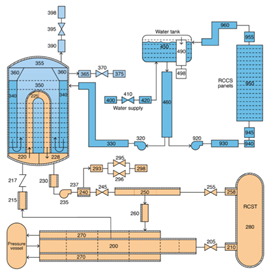
\includegraphics[width=10cm]{Figures/HTTF_RELAP_Nodalization.png}
    	\caption{\acrshort{httf} system nodalization scheme }
    	\label{fig:HTTF_RELAP_Nodalization}
    	\end{center}
\end{figure}

\subsubsection{Input model for \acrshort{httf}}

Figure \ref{fig:HTTF_RELAP_RPV_Nodalization_Axial} shows the axial \acrshort{rpv} \acrshort{r5} nodalization. To summarize, flow enters from the cold duct (270), passes through the core support structure (105) under the outlet plenum bottom plate, then flows up through an annulus (115) between the primary pressure vessel and core barrel to the inlet plenum (120). Flow then passes down through various flow channels (132, 140, 145, 150, 162, 164, 166) in the core and reflectors, recombines in the outlet plenum (175), then flows out into the hot duct (200). It is volumes 175 and 190 that are to be replicated using \acrshort{cfd}. More details about the axial nodalization can be found in Sections 4.1 and 5.1 of Bayless’ input model.

\begin{figure}
    \begin{center}
    	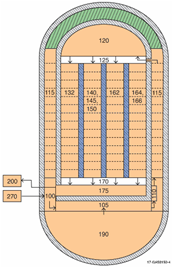
\includegraphics[width=8cm]{Figures/HTTF_RELAP_RPV_Nodalization_Axial.png}
    	\caption{Axial nodalization diagram of the \acrshort{httf} \acrshort{rpv}}
    	\label{fig:HTTF_RELAP_RPV_Nodalization_Axial}
    	\end{center}
\end{figure}

Figure \ref{fig:HTTF_RELAP_RPV_Nodalization_Radial} shows the radial \acrshort{rpv} geometric nodalization. More details about how this geometry is represented as \acrshort{r5} volumes and junctions can be found in 5.1 of Bayless’ input model. The central reflector is divided into three regions consisting of a central solid cylinder, a middle ring of ceramic consisting of six channels, and a solid outer ring that is adjacent to the core. This core ring is divided into three fueled rings to replicate the hexagonal block pattern of the modular high-temperature gas-cooled reactor, which has three fueled rings. Figure 4 shows which blocks are included in each of the rings in a 60-degree sector; the boundaries of the inner and outer rings were extended beyond the full hexagonal block geometry to include all of the coolant channels. Each fueled ring consists of hexagonal blocks, which have heater rods embedded and various number of coolant channels. The side reflector encapsulates the outermost fueled ring; it consists of three separate rings. The innermost ring is solid ceramic, the middle ring consists of channels, and the outermost is a relatively thin solid ring of ceramic. A small coolant gap exists between this outermost side reflector and the permanent reflector. Another small coolant gap surrounds the permanent reflector. The permanent reflector is in direct contact with the core barrel.

\begin{figure}
    \begin{center}
    	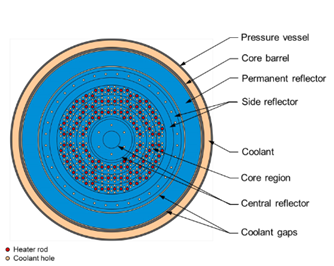
\includegraphics[width=10cm]{Figures/HTTF_RELAP_RPV_Nodalization_Radial.png}
    	\caption{Radial nodalization diagram of \acrshort{rpv}}
    	\label{fig:HTTF_RELAP_RPV_Nodalization_Radial}
    	\end{center}
\end{figure}

\subsection{Previous \acrshort{httf} \acrshort{r5} Simulations}

Significant work has been done in order to model the system response of the \acrshort{httf} using \acrshort{r5} for different testing scenarios. In 2019, \acrshort{osu} performed a transient test that simulated a double ended inlet-outlet crossover duct break, a type of depressurized conduction cooldown test [13]. Epiney [14] utilized \acrshort{r5} to model this test, and compared the simulation results to measured test data. The input deck for the test was first prepared by modifying Bayless’ base \acrshort{httf} \acrshort{r5} deck to incorporate additional nodalization in the outlet plenum and hot duct (since \acrshort{r5} cannot simulate countercurrent flow within a single volume), as well as initial conditions and modified trips and controls, with the use of Python helper tools. These tools also extract and plot information from the output as well as the measured data. 

The results were that ceramic and helium temperatures, as well as heat removal rates after the duct break, were generally underpredicted, with many assessment findings being minimal or insufficient in agreement with the test data. A lack of helium flow and uncertainty in material data (i.e. helium leaks, cold helium injections, uncertainty in material emissivities and friction factors) prevents troubleshooting problems with the input deck; these problems appear to lead to the energy balance within the core not being properly captured. This leads to important phenomena such as natural circulation and molecular diffusion—two phenomena that were predicted through scaling laws—were not observed as expected.

\section{\acrshort{fvm} Solvers}

The use of commercial \acrshort{cfd} codes has led to leaps in engineering fields that require detailed modelling of fluid flow and heat transfer, particularly in the power generation and aerospace sectors. With respect to nuclear, guidance has been written on how to use \acrshort{cfd} for general safety analysis \cite{johnson_pointer}, and has been used to improve power outputs at existing nuclear power plants \cite{wang_wang_tian_qiu_su_2021} via modelling complicated geometries within the core, and finding ways to enhance turbulent mixing. In the \acrshort{httf} \acrshort{lp}, the walls and support columns create disturbances in the flow, resulting in eddies and wakes (see Figure \ref{fig:LP_Flow_Behavior}).
\begin{figure}[!ht]
    \begin{center}
    	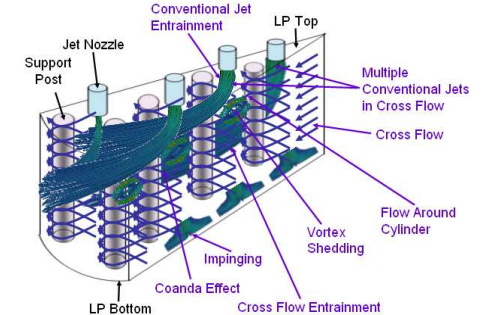
\includegraphics[width=13cm]{Figures/Flow_Behavior_LP.PNG}
    	\caption{Different types of fluid behaviors that might be seen in a typical \acrshort{htgr} \acrshort{lp} \cite{rodriguez_2010}}
    	\label{fig:LP_Flow_Behavior}
    	\end{center}
\end{figure}
The following subsections briefly describe the general equations that are solved (specifically, in \acrshort{star} and the general workflow of create a geometry, a mesh, and selecting the appropriate physics for the problem at hand.

\subsection{Fundamental Equations}

In order to represent fluid flow accurate, the fluid must be regarded as a continuum, implying that a single fluid “element” does not account for the individual motions or structure of a fluid molecule. This allows the fluid to be modelled according to macroscopic parameters such as temperature, velocity, pressure, and density, as well as spatial and temporal derivatives. This fluid, and the mechanics by which it behaves, must obey the three conservation laws:

\begin{itemize}
    \item The mass of the fluid must be conserved;
    \item The rate of change of (linear and angular) momentum equals the sum of the forces on a fluid particles (Newton’s second law);
    \item The rate of change of energy is equal to the sum of the rate of heat addition to and the rate of work done on a fluid particle (first law of thermodynamics)
\end{itemize}

These three principles, which describe classical continuum mechanics, are described in equation form in <Reference Appendix B equations>. There appears to be a similar pattern with respect to how these equations are written which, if rewritten in terms of some general variable $\phi$:

\begin{equation}
    \frac{\partial (\rho \phi)}{\partial t} + \nabla \cdot (\rho \phi \overrightarrow{v}) = \nabla \cdot (\Gamma \nabla \phi) + S_{\phi}
\label{eq:GTE_Differential}
\end{equation}

Equation \ref{eq:GTE_Differential} is the differential transport equation for property $\phi$. By setting $\phi$ equal to 1, $\overrightarrow{v}$ (which has scalar components $u$, $v$, $w$), and $E$, can be solved via the equations outlined in Appendix B. \acrshort{cfd} codes that use the \acrshort{fvm} typically take this transport equation and manipulate it such that it is written in integral form. By integrating \ref{eq:GTE_Differential} across a control volume, and applying Gauss's divergence theorem, \ref{eq:GTE_Differential} becomes:

\begin{equation}
    \frac{\partial}{\partial t} \int\limits_{CV} \, (\rho \phi) dV\ + \int\limits_{CS} \, \overrightarrow{n} \cdot (\rho \overrightarrow{v} \phi) dA\ = \int\limits_{CV} \, \overrightarrow{n} \cdot (\Gamma \nabla \phi) dA\ + \int\limits_{CV} \, S_{\phi} dV\
\label{eq:GTE_Integrated}
\end{equation}

Equation \ref{eq:GTE_Integrated} translates to:

\begin{figure}[!ht]
    \begin{center}
    	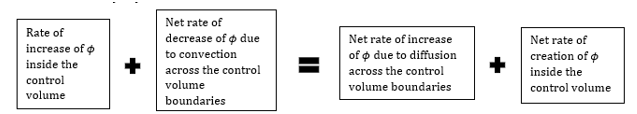
\includegraphics[width=13cm]{Figures/GTE_Balance.PNG}
    	\caption{Balance of $\phi$ via Equation \ref{eq:GTE_Integrated}}
    	\label{fig:GTE_Balance}
    	\end{center}
\end{figure}

\acrshort{cfd} software (ANSYS Fluent, OpenFoam, STAR-CCM+) use finite volume domain spatial discretization in order to subdivide a domain into a specific number of control volumes. These individual control volumes are called mesh cells, and may vary in size and shape. Different numerical techniques are used to model each term (e.g. upwind schemes for convective terms, implicit for unsteady flows, central differencing for diffusion terms). The selection of the numerical solver for each term is dependent on what type of problem needs to be solved. \acrshort{star} is used for this analysis.

\subsection{Geometry and Mesh}

In \acrshort{star}, a geometry is the starting point for all simulation efforts, and is typically in the form of a CAD model. Geometries can be modified with \acrshort{star}'s own CAD model modifier, and can be used to represent either the places where fluid is not supposed to be (e.g. walls of a fluid domain), or the fluid domain itself. The user then must then assign this geometry into sections, or parts, and these parts to a region. A region is a volume domain which is completed surrounded by boundaries, and is the domain where physics takes place. Regions must be created prior to creating a mesh, and regions contain information about the boundary conditions of the problem. Multiple regions can be created that utilize different models and solvers, but often, one class of solvers is applied to all regions.

Once a region has been created, the user must create a mesh. A mesh is a domain that has cells which store information about the variables being solved. Meshes, in \acrshort{star}, can be region- or parts-based. Both methods permit the user to specify certain locations of the continua where higher or lower fidelity is needed based on what the flow characteristics might be. Region-based meshing practices have been phased out with later versions of \acrshort{star}, so the suggested practice was to utilize operations on the parts generated from the CAD model to automatically generate the mesh. \acrshort{star} provides the user flexibility in what type of meshes can be generated, as well as optimization tools to improve individual cell quality, skewness angles, and aspect ratios. These automation tools save the user considerable amounts of time, particularly when trying to mesh the near-wall regions, because a user can run a coarse mesh to convergence, reduce the base size of the cells, and run another simulation that will likely converge more quickly. More information about specific strategies for meshing the \acrshort{httf} \acrshort{lp} can be found in Section !need reference to Mesh section!.

\subsection{Fluid Flow Models}

The type of solver that is used to solve \ref{eq:GTE_Integrated} depends on the types of physics that the user wants to specify, as well as how well the solution converges. The more assumptions that are made and implemented into the solvers (e.g. incompressible, subsonic, steady, inviscid), the less terms there are in \ref{eq:GTE_Integrated} to be solved for, and the faster the solver will iterate.

Information about the workflow for choosing the proper solver for simulations involving gases is outlined in detail in \cite{cd-adapco}, but the general steps are after creating the mesh:
\begin{itemize}
    \item Determine if the fluid is Newtonian or non-Newtonian;
    \item Select a steady or transient time mode;
    \item Choose a solver strategy (coupled, segregated, viscous):
    \begin{itemize}
        \item Coupled flow: solves \acrshort{ns} equations simultaneously with pseudo-time-stepping approach;
        \item Segregated flow: similar to coupled flow, but solves the momentum equations sequentially; solves \ref{STAR_Energy} for some alternate variable besides total energy $E$ depending on the model:
        \begin{item}
            \item Segregated fluid enthalpy: solves for fluid chemical thermal enthalpy $i$, then fluid temperature $T$ via \acrshort{eos};
            \item Segregated fluid isothermal: $T$ is kept constant;
            \item Segregated fluid temperature: solves for $T$.
        \end{item}
    \end{itemize}
    \item Viscous regime (inviscid, laminar, turbulent)
    \item Specify fluid \acrshort{eos} (constant density, ideal gas, thermal non-equilibrium, custom)
    \item Set various under-relaxation factors;
\end{itemize}

The $Ma$ number was initially suspected to be less than 0.2, even if a \acrshort{pcs} \acrshort{mfr} was assumed to be close to 100 g/s. According to \cite{cd-adapco}, a segregated flow model is suggested since the fluid is assumed to be incompressible. This model is detailed more in Section !Need to reference Segregated Flow Model Section!.

\subsection{Turbulence Modelling}

There is no set definition of what turbulence is; rather, it is better defined by general flow characteristics and features. Turbulent flows are unsteady, irregular, seemingly random and chaotic; its motions can be observed at many scaled from eddies and bulges comparable in size to the width the flow container to the smallest scales that a camera can resolve [8]. 

This latter point is particularly important because it is the basis by which various assumptions can be made that form lead to different turbulent models. These models are substitutes for directly solving the \acrlong{ns} (\acrshort{ns}) equations for turbulent flow (known as \acrlong{dns}, or \acrshort{dns}), by which required numerical power to simulate turbulent flows grows as a cube of the $Re$ number. \acrshort{dns} can be used for modelling small geometries such as the hottest channel, but it is not feasible for an entire coolant system, such as the \acrshort{lp} domain that is to be simulated.

\subsection{\acrlong{rans}}

\acrshort{star} has two classes of turbulence models: \acrlong{rans} (\acrshort{rans}), and scale-resolving simulations. \acrshort{rans} utilizes Reynolds decomposition, which divides the transport scalar into both a mean ($\overline{\phi}$) and fluctuating ($\phi^{'}$) components (\ref{eq:Reynolds_Decomposition}), with emphasis on solving for the mean transport scalar using a variety of closure models. 

\begin{equation}
    \phi(t) = \overline{\phi} + \phi^{'}
\label{eq:Reynolds_Decomposition}
\end{equation}

By contrast, the scale-resolving simulations resolve large scales of turbulence, and models small-scale motions.  Previous attempts at modelling phenomena in the \acrshort{lp} have utilized \acrshort{rans} methods, which will be the focus of this section, and is chosen for these simulations.

In \acrshort{rans}, the averaging process may be thought of as time-averaging for \acrshort{ss} situations and ensemble averaging for repeatable transient situations. Inserting the decomposed solution variables into the \acrshort{ns} equations results in continuity and momentum equations for the mean quantities representing the Reynolds-averaged \acrshort{ns} equations (see Appendix A, Equations \ref{RANS_Continuity} through \ref{RANS_z_Momentum}), which can be condensed into another transport equation for scalar $\psi$. 

\begin{equation}
    \frac{\partial \Phi}{\partial t} + \nabla \cdot (\varphi \overrightarrow{U}) = \frac{1}{\rho} \nabla \cdot (\Gamma_{\varphi} \nabla \Phi) + \left [  \frac{\partial (\overline{u^{'} \varphi^{'}})}{\partial x} + \frac{\partial (\overline{v^{'} \varphi^{'}})}{\partial y} \frac{\partial (\overline{w^{'} \varphi^{'}})}{\partial z} \right ] + S_{\Phi}
\label{eq:STAR_Turbulent_Transport}
\end{equation}

Equation \ref{eq:STAR_Turbulent_Transport} assumes incompressible flow with a fluid continuum that has a constant viscosity. This equation focuses on the mean flow and the effects of the Reynolds stresses on the mean flow properties. Fluctuations in pressure and velocity are not very significant on the final results unless the Mach number approaches 3-5 according to an analysis performed by Bradshaw \emph{et al.} \cite{bradshaw_cebeci_whitelaw_1981}; the \acrshort{httf} \acrshort{lp} does not come close to this limit.

\subsection{Wall Treatment}

Flows, whether turbulent are not, can be either fully-developed or not. Fully-developed implies that the velocity and temperature gradients within the flow do not change over the course of some distance \cite{white_2008}. The region where these gradients exist is called the boundary layer \cite{liburdy_2021}. An obstacle can disturb this fully-developed flow and cause changes to these gradients by imposing both a force normal to the fluid velocity vector (e.g. impingement) and tangential to it (shear stress). These two effects will impact the pressure drop along the fluid direction (also termed the entry length), as pressure drop is typically linear with respect to distance in a fully developed flow. The deviance of the velocity vectors from the mean flow direction implies that, for turbulent flows, there will be eddies. The existence of these eddies helps mix fluid streams of different temperatures and mass compositions.

\begin{figure}[!ht]
    \begin{center}
    	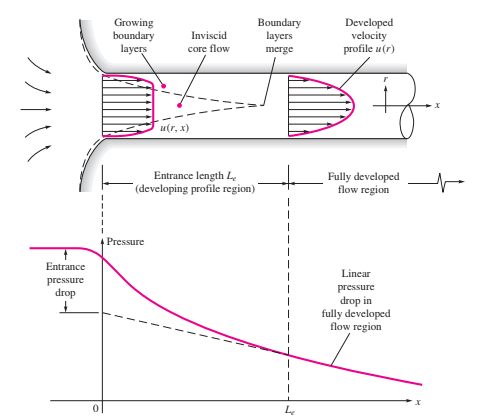
\includegraphics[width=13cm]{Figures/Developing_Flow.PNG}
    	\caption{Illustration of the entry-length and fully developed flows in a circular pipe \cite{white_2008}}
    	\label{fig:white_2008}
    	\end{center}
\end{figure}

The mesh must be modified to accurately capture how these wall shear stresses affect the fluid equation of state (\acrshort{eos}). A quantification of how viscous effects (e.g. tangential forces) compare to the overall behavior of the flow (which is determined from both viscous and inertial forces far from the wall) is needed. The $Re$ number is a dimensionless number that quantifies this proportion of this force:

\begin{equation}
    Re = \frac{U_{\infty} y}{\nu} \equiv \frac{Inertial Forces}{Viscous Forces}
\label{eq:Re_Number}
\end{equation}

Where $y$ is the normal distance from the wall into the fluid. If $y$ approaches zero, the $Re$ approaches 1, and the viscous forces will be the same magnitude as the inertia forces. This implies that there exists a thin layer near the wall where viscous effects influences the velocity profile significantly more than the inertia forces. This definition of the $Re$ can be modified if the mean flow velocity, $\overline{U}$, is strictly a function of the normal distance $y$, the fluid dynamic viscosity $\mu$, and the wall shear stress, $\tau_{w}$:

\begin{equation}
    \overline{U} = f(y,\rho,\mu,\tau_{w})
\label{eq:Viscous_Mean_Velocity}
\end{equation}

To get this in a form similar to \ref{eq:Re_Number}, a substitution can be made for $\tau_{w}$ such that it is a function of the "friction velocity" $u_{\tau}$:

\begin{equation}
    u_{\tau} = \sqrt{\tau_{w}/\rho}
\label{eq:Mean_Velocity_Viscous}
\end{equation}

Since $u_{\tau}$ has units of velocity, it can be used in dimensional analysis to generate a nondimensional velocity $u^{+}$:

\begin{equation}
    u^{+} = \frac{\overline{U}}{u_{\tau}} = f \left (\frac{\rho u_{\tau} y}{\mu} \right ) = f(y^{+})
\label{eq:u_star_viscous}
\end{equation}

To account for the region that is impacted by the shear stress of the wall, but is not dependent on the viscosity of the fluid, the mean velocity can be a function of the boundary layer thickness $\delta$ instead:

\begin{equation}
    \overline{U} = f(y,\rho,\delta,\tau_{w})
\label{eq:Mean_Velocity_Inertial}
\end{equation}

Dimensional analysis would then show that:

\begin{equation}
    u^{+} = \frac{\overline{U}}{u_{\tau}} = f \left (\frac{y}{\delta} \right ) = f(y^{+})
\label{eq:u_star_inertial}
\end{equation}

This relationship, that $u^{+}=f(y^{+})$, can be used to describe a class of flows at different points from the wall. The two regions of interest are the viscous sub-layer, by which the $\overline{U}$ is dominated by viscous forces (\ref{eq:u_star_viscous}), where $y^{+}<5$, and the inertia-dominated layer (\ref{eq:u_star_inertial}), where $y^{+}>30$. These different layers are shown in \ref{fig:Velocity_Layers}. 

\begin{figure}[!ht]
    \begin{center}
    	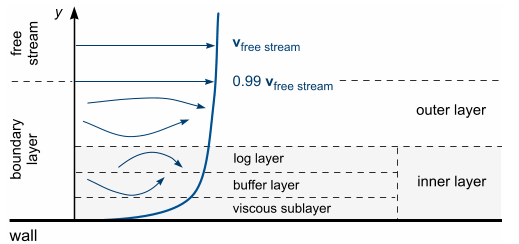
\includegraphics[width=13cm]{Figures/Velocity_Layers.PNG}
    	\caption{Visualization of the three regions for wall treatment \cite{cd-adapco}}
    	\label{fig:Velocity_Layers}
    	\end{center}
\end{figure}

Experiments have been performed to characterize how $u^{+}$ relates to $y^{+}$. It turns out, that for the viscous sub-layer, $u^{+} \propto y^{+}$, implying a linear relationship, whereas for the inertial region, the relationship is logarithmic:

\begin{equation}
    u^{+} \propto \frac{1}{\kappa} \ln{E y^{+}}
\label{eq:Inertial_Region_Relation}
\end{equation}

Here, $E$ is a constant depending on the wall roughness, and $\kappa$ (von Karman's constant) is a universal constant equal to about 0.4. The significance of these relations is that, for a whole range of flow geometries and $Re$, these relations will hold. This is important because these relations can be provided as tools to ensuring that the mesh is set up to have $y^{+}$ values either in the viscous sublayer or the inertia region, and that the appropriate wall-treatment models are selected (two-layer, high $y^{+}$, low $y^{+}$) such that $y^{+}$ values do not fall between 5 and 30 (also known as the buffer layer).

\begin{figure}[!ht]
    \begin{center}
    	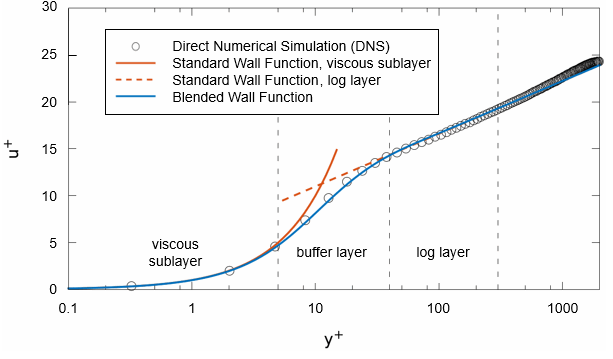
\includegraphics[width=13cm]{Figures/Velocity_Distribution_Layers.PNG}
    	\caption{$u^{+}$ distribution near a solid wall for turbulent flows \cite{cd-adapco}}
    	\label{fig:Velocity_Distribution_Layers}
    	\end{center}
\end{figure}



\section{\acrshort{vandv} Description}

The concern of \acrshort{vandv} is to assess the accuracy of a computational simulation, whether the simulation pertains to \acrshort{cfd} or computational heat transfer (CHT). Formal guidance on how to go about performing \acrshort{vandv} is set out in ASME \acrshort{vandv} 20-2009 \cite{vandv}, which will be used in preparation of simulation results. In order to properly present results, it is important to not only report findings within the body of this report, but also in other documents. The results of the simulations ran, and comparison to experimental data, will be published as appendices to this report.

Verification is the process of determining that a model implementation accurately represents the developer’s conceptual description of the model and the solution to the model (“did I do the thing right?”) Code and solution verification precede validation; it establishes that the code accurately solves the mathematical model incorporated in the code (i.e. the code is free of mistakes for the simulations of interest). It involves quantification of errors, including:

\begin{itemize}
    \item Roundoff error: comparing results obtained using different levels of machine accuracy, such as single and double precision;
    \item Iterative convergence error: investigating the effects of systematic variation of the truncation criteria for all residuals on target quantities of interest;
    \item Discretization error: requiring at least three successive levels of mesh refinement
\end{itemize}

Validation is the process of determining the degree to which a model is an accurate representation of the real world from the perspective of the intended uses of the model (“did I do the right thing?”) In short, validation cannot occur without experimental data with which to compare the result of the simulation. It involves the quantification different types of uncertainties, including:

\begin{itemize}
    \item Input uncertainty: estimated by means of a sensitivity or uncertainty analysis, involving multiple test runs of the model with different values of input data samples from probability distributions based on their mean value and expected variations
    \item Physical modelling uncertainty: directly comparing \acrshort{cfd} results with high-quality experimental results
\end{itemize}

The discrepancy between the experimental data and the simulation results, $E$, is the difference between the simulation result and the data value:

\begin{equation}
    E = S - D
\label{eq:Discrepancy_Equation}
\end{equation}

In terms of errors, $E$ is the difference between the simulation and experimental errors:

\begin{equation}
    E = \epsilon_{s}-\epsilon_{d}
\label{eq:Sim_Exp_Error}
\end{equation}

The errors of the simulation $\epsilon_{sim}$ is quantified as the sum of the model assumptions (e.g. the physics that is assumed for the particular problem) $\epsilon_{model}$, the input errors (e.g. \acrshort{bc}'s) $\epsilon_{input}$, and the numerical errors from solving the given set of equations $\epsilon_{num}$:

\begin{equation}
    \epsilon_{sim} = \epsilon_{model} + \epsilon_{input} + \epsilon_{num}
\label{eq:Sim_Error_Quantified}
\end{equation}

Since the input, numerical, and experimental errors are often not known (and neither are their uncertainties), it is best to quantify these as the validation standard uncertainty $u_{val}$ so that $\epsilon_{model}=E \pm u_{val}$. This assumption assumed that these errors are dispersed around a population mean \cite{TestUncertainty}. Coleman and Stern \cite{coleman_stern_1997} define this validation uncertainty as the square root of the sum of the squares of the numerical, input, and data uncertainties:

\begin{equation}
    u_{val} = \sqrt{u_{num}^{2} + u_{inp}^{2} + u_{d}^{2}}
\label{eq:Validation_Uncertainty}
\end{equation}

$u_{num}$ can be approximated via conducting a grid independence study, specifically by using Roache's Grid Convergence Index \cite{vandv}. This parameter ($GCI$) is a measure of the percentage the computed value is away from the value of the asymptotic numerical value \cite{slater_2021}. As the grid is refined (grid cells become smaller and the number of cells in the flow domain increase) and the time step is refined (reduced) the spatial and temporal discretization errors, respectively, should asymptotically approach zero, excluding computer round-off error. Since this study only pertains to examining the results at one time step, the temporal error can be ignored, so the study (which utilizes Richardson's extrapolation method) only pertains to quantifying the discretization error. $u_{num}$ can be approximated as half of the grid convergence index 


%-------------------MATERIALS & METHODS--------------------------

\chapter{Materials and Methods}

\section{\acrshort{r5} Simulations}

\acrshort{r5} (\acrshort{r5}) was used to generate the \acrshort{bc}'s for the \acrshort{star} \acrshort{lp} simulation. The specific time chosen to simulate the test was chosen at 5000 seconds, because it most closely resembles a \acrshort{ss} when looking at various temperature and pressure readings throughout the system (see Figures  through ), and is the closest that the core arrives at some sort of \acrshort{ss} condition. The \acrshort{bc}'s that were applied to the \acrshort{lp} simulation were:

\begin{itemize}
    \item Inlet \acrshort{mfr} and fluid temperature (from branch 170)
    \item Outlet pressure (from pipe 215)
    \item Wall temperatures (various heat structures), include 1200-001 (\acrshort{hd}), 1320-014 (\acrshort{lp} roof), 1660-015 (\acrshort{lp} walls), 1750-001 (\acrshort{lp} floor), 1751-001 (support posts), and 2150-001 (outlet duct)
\end{itemize}

\subsection{\acrshort{mfr} Approximations}

In order to be able to simulate the \acrshort{httf} in \acrshort{r5}, the \acrshort{mfr} had to be implemented into the \acrshort{httf} deck via a branch (235) and \acrshort{tdj} (237) component combination, since not enough information was provided by the vendor for circulator frictional torque and slippage. Since the \acrshort{osu} \acrshort{httf} is not equipped with a flow meter that explicitly estimates the primary loop’s \acrshort{mfr}, the pressure transducer readings (PT-6201 and PT-6202) were used to deduce the pressure drop across the circulator. With the pressure drop available, and a fifth-degree polynomial fitting scheme provided by the vendor, the volumetric flow rate was approximated. The \acrshort{mfr} was calculated by then using the thermocouple readings (\acrshort{tf}-6201 and \acrshort{tf}-6202) to determine the fluid density, and smoothed using RStudio (see Figure \ref{fig:Calculated_MFR}). All pressure and temperature readings from the test are provided in Figure \ref{fig:Circ_Inlet_Outlet_State}. 

\begin{figure}
    \begin{center}
    	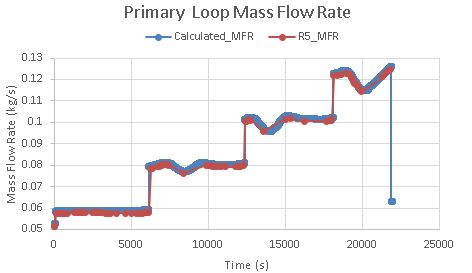
\includegraphics[width=10cm]{Figures/Calculated_MFR.JPG}
    	\caption{Calculated \acrshort{mfr} and implemented into \acrshort{r5}}
    	\label{fig:Calculated_MFR}
    	\end{center}
\end{figure}

\begin{figure}
    \begin{center}
    	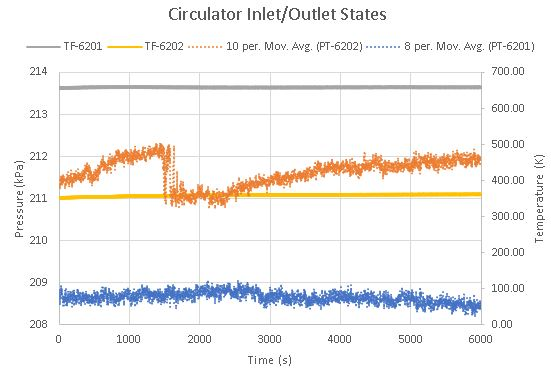
\includegraphics[width=10cm]{Figures/Circ_Inlet_Outlet_State.JPG}
    	\caption{Experimental data for circulator inlet/outlet temperature and pressure readings used for generating \ref{fig:Calculated_MFR}}
    	\label{fig:Circ_Inlet_Outlet_State}
    	\end{center}
\end{figure}

Likewise, these instrument readings allowed the capability to calculate the specific enthalpy (using Engineering Equation Solver) to determine the \acrshort{mfr} based on mass flow calorimetry (see Equation ). At \acrshort{ss}, the heat rate into the system (estimated to be that provided by the heaters) should be what is removed, if ignoring the radiative heat transfer from the \acrshort{rpv} to the \acrshort{rccs}. 

\subsection{Description of \acrshort{r5} Simulations}

Several iterations were performed in order to attempt to converge some of the system level parameters with the experimental data. The two main approaches were to simulate the heat-up phase to a \acrshort{ss}, then simulate the experiment up to 5000 seconds, and obtaining the \acrshort{ss} conditions directly at 5000 seconds. Specific modifications are discussed below. 

\subsection{Iteration 1}

The first approach was to directly simulate the test with the initial conditions specified directly in the experimental data, with no heat-up phase. A \acrshort{mfr} was approximated using the pressure 
Likewise, since round of simulations involved minimal changes to Paul Bayless’ QA deck, except for modifying the 235 pump component into a branch (235) and \acrshort{tdj} component (237). The \acrshort{tdj} component 


\subsection{Iteration 2}

The second iteration of tests (presented at the ANS conference) attempted to test flow rates that were substantially less than what was initially calculated (0.25x-0.625x of nominal), as well as attempting to simulate the heat-up phase and performing the test through 8000 seconds. 8000 seconds was chosen to show the audience whether or not the system changes via a step change in mass flow rates was simulated realistically. 

\subsection{Iteration 3}

The third iteration of tests utilized a limited range of flow rates (0.3125x, 0.375x, 0.4x, 0.4375x of nominal), as well as making some changes to the \acrshort{r5} base deck, including:
\begin{itemize}
    \item Controlling primary system pressure by removing the two valves 295 and 296, removed branch 293, converted single volume 298 into a \acrshort{tdv} that simulated what is already in general table 220;
    \item Increasing the forward loss coefficients for volumes 100, 105, 110, 115, 175, 183, and 270 to better approximate the pressure losses in the \acrshort{rpv}, as well as the \acrshort{sg} tubes, 225;
    \item Writing initial deck to start from ~99\% \acrshort{sg} level, drain to 30\%, then had restart deck that started from same level and drained to ~69\%. Subsequent restart deck would simulate the actual test until \acrshort{sg} level dropped to ~49\%; and
    \item Adjusting the thermal conductivity (reduced by a factor of ~10) of the \acrshort{sg} tubes to reduce the temperature difference across the core and justify this as fouling;
\end{itemize}

While it appeared that the pressure losses through the system were closer to what was measured experimentally, the results from these simulations were not used because the \acrshort{mfr} through the 170 volume were negative (implying reverse or stagnant flow) and the numerous changes performed were not justified by the QA calculations, particularly the loss coefficients.  

\subsection{Iteration 4}

The fourth iteration incorporating using the base deck, but only implementing an artificial volume (298) to control the system pressure and temperature after the circulator. Likewise, both a \acrshort{ss} calculation was performed at 5000 seconds, and the heat-up phase/test was simulated up to 5000 seconds. 


\section{\acrshort{star} Simulations}

Simulation results from \acrshort{r5} were then provided into the \acrshort{star} \acrshort{lp} model in the form of boundary conditions. This chapter, and its subsections, elaborates more about the geometry, mesh, and physics used to model the \acrshort{lp}.

\subsection{Geometry}

The boundaries of the simulation domain were first determined before performing any simulations. Previous \acrshort{star} models for the \acrshort{lp} drew the inlet boundary at the interface between the \acrshort{lp} fluid domain and the \acrshort{lp} roof, while the outlet boundary was drawn somewhere in the outlet duct. These boundaries defining the fluid domain were redrawn. (see Figure \ref{fig:LP_Geometry} for the full model). The inlet boundary was determined as the point where the multiple junction 170 in \acrshort{r5} exists because the flow profile into the \acrshort{lp} fluid domain is not fully developed when it enters that domain, since the channel cross section shape changes from round holes to "crescents" (see Figure \ref{fig:LP_Inlet_Crescents}). The tee that joins the \acrshort{od} with the \acrshort{sg} inlet was incorporates, as this would influence the velocity profile of the helium jets exiting the \acrshort{lp}. Additionally, the pipe that connects the \acrshort{pcs} with the \acrshort{rccs} was included (up to the place where the valve exists) because, while the fluid in this domain is stationary, the behavior of the jets of fluid that impinge upon it (as well as the heat transfer) would be different if it did not exist.  

The final CAD design had four main parts, each having a different level of fidelity when it came to the mesh. These include:

\begin{itemize}
    \item \acrshort{lp} 
    \item \acrshort{hd}
    \item Tee
    \item Pipe connecting the tee to where the \acrshort{rcst} valve would be (Connection2RCST)
\end{itemize}


\begin{figure}[!ht]
    \begin{center}
    	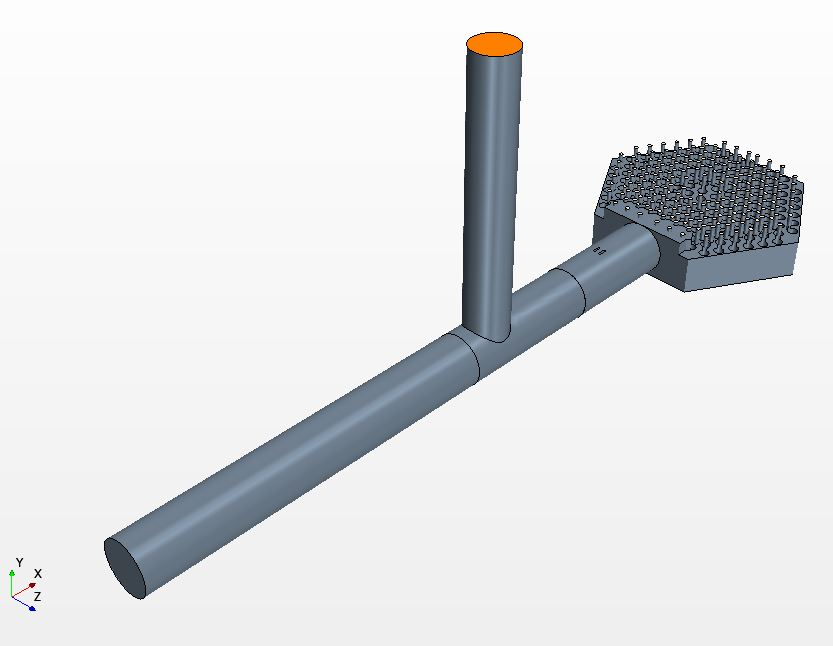
\includegraphics[width=10cm]{Figures/LP_Geometry.JPG}
    	\caption{Geometric model used for creating parts in \acrshort{star}}
    	\label{fig:LP_Geometry}
    	\end{center}
\end{figure}

\begin{figure}[!ht]
    \begin{center}
    	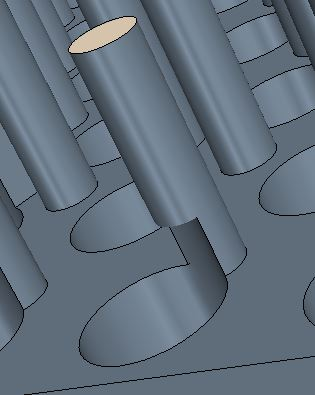
\includegraphics[width=5cm]{Figures/LP_Inlet_Crescents.JPG}
    	\caption{Inlet channel cross section changes from circular to crescent-shaped}
    	\label{fig:LP_Inlet_Crescents}
    	\end{center}
\end{figure}

\subsection{Mesh}

Parts-based meshing was used to mesh the four individual parts with different levels of fidelity. The \acrshort{lp} and \acrshort{hd} would both have jet impingement from the walls and wake formation from the support columns and the rakes. Likewise, the most complex phenomena in the tee is that the mean fluid velocity vector would be shifting direction by 90 degrees, and would impinge upon the stagnant fluid existing in the Connection2RCST part. The Connection2RCST was included because the form loss may be different than if it was not included, and a cap was applied to the end of the tee. 

Each of the four parts were meshed with triangular tetrahedrals, as this provided the best cell parameters that define a good mesh (particularly cell quality and aspect ratio, see Figure ...). \acrshort{star} provides the capability to use polyhedrals, but it was found that this often resulted in divergent solutions. The three meshes had 1.570+07, 2.323e+07 Table 

\begin{table}[!ht]\centering
\abovedisplayskip=0pt
\belowdisplayskip=0pt
\begin{tabular}{ m{4cm} m{4cm} m{4cm} }\hline
Model & Part & Number of Cells \\
Coarse & Lower Plenum & 1000000 \\
Coarse & Hot Duct & 1000000 \\
Coarse & Tee & 1000000 \\
Coarse & Connection2RCST & Need This \\
Middle & Lower Plenum & 1.445e+07 \\
Middle & Hot Duct & 1.159e+06 \\
Middle & Tee & 5.863e+04 \\
Middle & Connection2RCST & 2.524e+04 \\
Fine & Lower Plenum & 1.713134e+07  \\
Fine & Hot Duct & 4.285830e+06 \\
Fine & Tee & 1.766366e+06 \\
Fine & Connection2RCST & 4.518900e+04 \\
\hline\end{tabular}\caption{Number of cells present in each of the three \acrshort{star} models}\label{Number_Cells_STAR_Model}\end{table}

As previously stated, three different meshes had to be constructed in order to perform \acrshort{vandv} and properly capture the \acrshort{gci}. The number of 

\subsection{Physics}

As outlined in the literature review, an understanding of the physics that are hypothetically supposed to occur is important to ensure that parameters such as turbulent kinetic energy and dissipation are properly approximated in order to simulate a reasonable pressure drop and heat transfer.

The following models were used for all fluid domains:
\begin{itemize}
    \item Steady
    \item Ideal gas
    \item Three-dimensional
    \item Segregated flow (segregated fluid temperature)
    \item K-Epsilon Turbulence (low -Re)
    \item Low y+ Wall treatment
\end{itemize}

\ref{STAR_Conservation_of_Mass} through \ref{STAR_Energy} constitute the \acrshort{ns} equations fundamental to all flow regimes, while \ref{RANS_Continuity} through \ref{RANS_z_Momentum} represent the \acrshort{rans} turbulent equations that are to be solved for incompressible flow with constant velocity. These equations are what are solved based on the assumption that the pressure and viscosity differences in the \acrshort{lp} domain are small. Pressure can be assumed to be relatively constant since the experimental data (specifically, the pressure readings from PT-3001 and PT-3002) indicate only a pressure drop on the order of 10's to 100's of Pascals. Although fluid jet temperatures differ by several hundred degrees, which has a profound impact on the (dynamic) viscosity, the assumption of constant viscosity greatly simplifies the governing equations and speeds up calculations. 

\subsubsection{Segregated Flow Model}

In the context of the \acrshort{pg}-28 test, the experimental data suggest that the pressure drop across the \acrshort{lp} and \acrshort{hd} is not large compared to the absolute pressure (implying incompressible flow, which must be validated with the Mach number), the boundaries of the domain are not isothermal, and that the $Re$, while not as high as what is supposed to be modeled in the \acrshort{httf} scaling document (need reference), suggests turbulent flow. Likewise, since the flow being modeled is for one instance in time, the steady-state option is selected.

\subsubsection{Turbulence Model}

When using \acrshort{rans} models, the effects of turbulence on the mean flow must be accounted for, e.g. how the Reynolds stresses and time-averaged scalar transport terms affect the flow. Additional models are needed to predict these stresses and transport terms. \acrshort{rans} models differ by the parameters that are calculated from various number of equations. 

However, further models are needed to be specified. \acrshort{star} has several \acrshort{rans} models, including the $k-\epsilon$, $k-\omega$, Reynolds stress, and Spalart-Allmaras models. Each of these models is supposed to be applied to a specific flow behavior:
\begin{itemize}
    \item $k-\epsilon$ works well in confined, circulating flows, and is the most widely used and validated model, and also requires two additional equations to solve for the turbulent kinetic energy $k$ and the turbulent dissipation rate $\epsilon$;
    \item $k-\omega$ provides superior performance for complex boundary layer flows under adverse pressure gradients and separations, and also requires two additional equations for \acrshort{tke} and turbulent frequency, $\omega$;
    \item \acrlong{rsm} (\acrshort{rsm}) the individual Reynolds stresses better than the $k-\epsilon$, and is typically used where complex strain fields and/or significant body forces on the fluid domain exist, and requires seven additional equations (most computationally expensive);
    \item Spalart-Allmaras performs well in external flows where adverse pressure gradients exist, and requires one additional equation to solve for a kinematic eddy viscosity, $\Tilde{\nu}$. 
\end{itemize}

Despite the $k-\omega$ model being well-suited for low-$Re$ turbulent flows (which is the flow regime during the \acrshort{pg}-28 test), previous \acrshort{star} simulations for the \acrshort{lp} have utilized $k-\epsilon$ because it provides the best convergence, and is still applicable to the confined-flow problem that is being simulated. It is documented that the $k-\epsilon$ overpredicts the turbulence shear stress, particularly in the presence of large pressure gradients, and overpredicts the levels of turbulence and heat transfer when in regions where there is jet impingement. However, both of these concerns are likely not significant, since the $Re$ is relatively low (on the order of $10^{3}$) and pressure drops are on the order of a $10^{2}-10^{3}$ Pascal. Both of the two-equation models tend to fail to include subtle interactions between turbulent stresses and mean flow when compared to the \acrshort{rsm}, but the \acrshort{rsm} is computationally intensive. 

\subsubsection{Wall Treatment}

Once the $k-\epsilon$ model was selected, attention turned to how to capture the wall effects. To summarize, walls affect the boundary layers of the flow regime which, in turn, affect the state of the fluid (both pressure and temperature). The regions close to the wall must be refined sufficiently in order to properly resolve viscosity and inertial effects close to the wall. Prism layers, which are tetrahedrals that increase in thickness further away from the wall, can be specified in \acrshort{star}.

Since the $Re$ number is relatively low in the \acrshort{lp} for the \acrshort{pg}-28 test, it is best to use a low-Re, low $y^{+}$ wall treatment method, implying that the $y^{+}$ values for all of the walls in the simulation domain should be less than 1. The inclusion of this model negates the need to specify a surface roughness on the boundaries. 

\section{Grid Independence Study}

The objective of a grid convergence study for a steady-state simulation is to provide insight into how (and if) the base size of the mesh affects the solution.

For this grid convergence study, the 

%------------------------RESULTS--------------------------------

\chapter{\acrshort{cfd} Results}


%-----------------------DISCUSSION--------------------------------

\chapter{Discussion}

This section discusses some reasons why the results between the simulations and the experimental data exists, as well as what can be done with further simulations to narrow down the possibilities for the discrepancies. Specifically, \acrshort{r5} should be used to simulate a shakedown test that characterizes the circulator performance, using \acrshort{star} and altered outlet pressure field to re-examine the velocity profiles at the \acrshort{rx}, and using a separate code with higher fidelity to model the core region. 

\section{Validate \acrshort{httf} \acrshort{r5} Model Loss Coefficients}

One step that can be taken to ensure that the physics are being properly modeled is by validating the \acrshort{pg}-02 test. The \acrshort{pg}-02 test was completed in February 2017, with the goal of measuring the forced flow pressure drops across important components and regions of the \acrshort{pcs}. The \acrshort{pcs} was filled with nitrogen gas, and the circulator was set at 20 different statepoints, with no heat being added to the system. 

Since orifices were used to generate a reduction in fluid pressure, the \acrshort{pcs} \acrshort{mfr} was calculated using the principle of the Venturi effect (see Figure \ref{fig:PG02_Flow_Rates}). This test is one of the few times where the \acrshort{mfr} was known to a certain degree, and this \acrshort{mfr} is a key unknown for modelling in the \acrshort{r5} \acrshort{httf} input deck. 

\begin{figure}
    \begin{center}
    	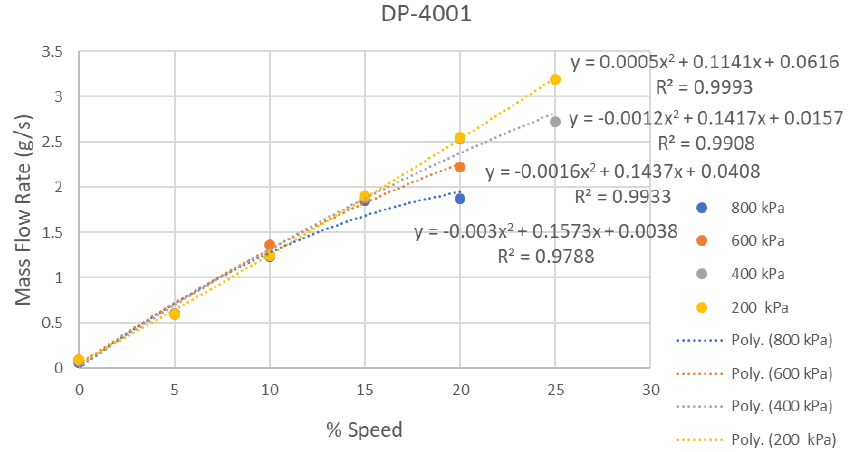
\includegraphics[width=12cm]{Figures/PG02_Flow_Rates.PNG}
    	\caption{The use of orifices permitted the calculation of the \acrshort{pcs} \acrshort{mfr} during the \acrshort{pg}-02 test}
    	\label{fig:PG02_Flow_Rates}
    	\end{center}
\end{figure}

The goal of this test would be to verify that the theoretical calculations for the forward loss coefficients originally calculated in the base deck are indeed correct, and concluding whether or not these coefficients are dependent on the Reynolds number. \acrshort{r5} provides capability to specify a Reynolds-number dependent loss coefficient.  These loss coefficients are particularly important because pressure has a strong effect on the thermodynamic state of the fluid, and accurately capturing these losses are important for conduction cooldown tests that need to be modeled, where the pressure losses (particularly across the core and in the plenums) have an effect on the time scales for flow reversal and onset of natural circulation. 

\section{Flow Physics Through \acrshort{r5} Core}

A fundamental assumption of Bayless' \acrshort{httf} \acrshort{r5} model is that the flow entering, transversing through, and exiting the \acrshort{rx} is uniform circumferentially (based on \ref{fig:HTTF_RELAP_RPV_Nodalization_Radial}), and that the characteristics differ in the radial direction. This assumption is inconsistent with the lumped-element model with equivalent circuits \cite{voldman_2022}. While this model is very simple considering the complex nature of the equations presented in Table \ref{STAR_NS_Eqn}, they do provide a general description of what the fluid might do. These equations essentially state that driving potential is equal to the product of some flow rate and the resistance for that flow to transverse between two points. In the context of fluids, the fluid pressure, $P$, is equal to the product of the volumetric flow rate $Q$ and the flow resistance, $R_{fluid}$.

Both the \acrshort{star} models and the experimental data indicate that the pressure field in the \acrshort{lp} is not uniform, and that the highest pressure occurs in regions furthest from the \acrshort{od}. In the \acrshort{r5} model, this is not shown because while the \acrshort{lp} is modelled with volumes 175, 185, 180, and 183 which permits a higher degree of fidelity as opposed to modelling the \acrshort{lp} domain with one branch (175), the "ring" model homogenizes the flow characteristics at each ring level, which includes both the fluid velocity and the fluid pressure. However, because the experimental data shows that the fluid pressure differs at the far end of the \acrshort{lp}, this will have an effect on the flow velocity and, consequently, the mass flow rate. This change in mass flow rate will also change the heat removed in each channel and, hence, the inlet jet temperatures.

Likewise, the inlet plenum is modelled as a single branch, and also does not factor in the changes in velocity and temperature of the fluid that enters the core region. Based on previous \acrshort{up} \acrshort{star} simulations performed by Dr. Gutowska \cite{gutowska_woods_cadell_2019}, the fluid velocities are not uniform circumferentially (see Figure <need figure>). This is problematic for the assumptions made in the \acrshort{r5} model, specifically when it comes to characterizing hot spots and, ultimately, the peak temperatures and where they occur. 

\section{Substituting \acrshort{r5} with a Higher Fidelity Solver}

\acrshort{inl}, through its \acrlong{moose} (\acrshort{moose}), has developed higher fidelity, finite element method solvers to tackle problems across a broad range of physics. Two codes that have been developed for subchannel analysis include \acrlong{r7} (\acrshort{r7}) \cite{zhang}, which builds upon the \acrshort{r5} infrastructure with multi-dimensional core analysis, and Pronghorn \cite{balestra_2019}. 

This, in tandem with the pressure field of the \acrshort{lp}, suggest that \acrshort{star} will need to be used to model both plenums, and that a higher fidelity solver will need to be used for modelling the \acrshort{rx} (such as RELAP7; see \cite{osti_1812877}). \acrshort{r5} may still be used to model the rest of the \acrshort{pcs} and the \acrshort{httf} loops. 

\chapter{Conclusion}

The objective of this investigation was to determine how well \acrshort{star} models the physics in the \acrshort{httf} \acrshort{lp}, within the inclusion of boundary conditions provided by Paul Bayless' \acrshort{r5} model, specific to the \acrshort{pg}-28 test completed in 2019, at the instance when the experimental data indicate a fairly steady state. This investigation is needed in order to see where and why differences occur before in both models before a complicated coupling scheme is used to couple both codes to model this specific test. Based on what was modeled, it is apparent that the highest uncertainty pertains to the boundary conditions being applied to \acrshort{star} (specifically, the inlet \acrshort{mfr} and temperatures, as well as the wall temperatures), which are derived from uncertainties in the loss coefficients supplied in the \acrshort{r5} and the flow physics modelled in the \acrshort{httf} \acrshort{rx}.


At best, \acrshort{r5} should be used for a general heat source and verifying that the heat balance is correct across the \acrshort{pcs}. 

\pagebreak

\bibliography{thesis}
\bibliographystyle{plain}

\pagebreak

\appendix

\chapter{Equations Solved in RELAP5-3D}

\begin{table}\centering
\abovedisplayskip=0pt
\belowdisplayskip=0pt
\begin{tabular}{ m{3cm} m{10cm} }\hline
Vapor Mass Continuity & {\begin{flalign}
\frac{\partial}{\partial t} (\alpha_{g} \rho_{g}) + \frac{1}{A} \frac{\partial}{\partial x} \left ( \alpha_{g} \rho_{g} v_{g} A \right ) = \Gamma_{g}&&
\label{R5_Vapor_Mass_Cont}\end{flalign}}\\[-2ex]
Noncondensable Vapor Mass Continuity & {\begin{flalign}
\frac{\partial}{\partial t} \left (\alpha_{g} \rho_{g} \chi_{n} \right ) + \frac{1}{A} \frac{\partial}{\partial x} \left ( \alpha_{g} \rho_{g} \chi_{n} v_{g} A \right ) = 0
\label{R5_Noncond_Vapor_Mass_Cont}\end{flalign}}\\[-2ex]
Liquid Mass Continuity & {\begin{flalign}
\frac{\partial}{\partial t} (\alpha_{f} \rho_{f}) + \frac{1}{A} \frac{\partial}{\partial x} \left ( \alpha_{f} \rho_{f} v_{f} A \right ) = \Gamma_{f}
\label{R5_Liquid_Mass_Cont}\end{flalign}}\\[-2ex]
Vapor Momentum & {\begin{flalign}
\begin{multlined}\alpha_{g} \rho_{g} A \frac{\partial v_{g}}{\partial t} + \frac{1}{2} \alpha_{g} \rho_{g} A \frac{\partial v_{g}}{\partial x} = -\alpha_{g} A \frac{\partial P}{\partial x} + \\ \alpha_{g} \rho_{g} B_{x} A - \alpha_{g} \rho_{g} A (\textbf{FWG})v_{g} + \Gamma_{g} A (v_{g,i}-v_{g}) - \\ \alpha_{g} \rho_{g} A (\textbf{FIG}) (v_{g}-v_{f} - C \alpha_{g} \alpha_{f} \rho_{m} A \left [ \frac{\partial (v_{g}-v_{f})}{\partial t} + v_{f} \frac{\partial v_{g}}{\partial x} - v_{g} \frac{\partial v_{f}}{\partial t} \right ] \end{multlined}&&
\label{R5_Liquid_Cont}\end{flalign}}\\
Liquid Momentum & {\begin{flalign}
\begin{multlined}\alpha_{f} \rho_{f} A \frac{\partial v_{f}}{\partial t} + \frac{1}{2} \alpha_{f} \rho_{f} A \frac{\partial v_{f}}{\partial x} = \\ -\alpha_{f} A \frac{\partial P}{\partial x} + \alpha_{f} \rho_{f} B_{x} A - \alpha_{g} \rho_{f} A (\textbf{FWF})v_{f} + \Gamma_{f} A (v_{f,i}-v_{f}) - \\ \alpha_{f} \rho_{f} A (\textbf{FIF}) (v_{f}-v_{g} - C \alpha_{g} \alpha_{f} \rho_{m} A \left [ \frac{\partial (v_{f}-v_{g})}{\partial t} + v_{g} \frac{\partial v_{f}}{\partial x} - v_{f} \frac{\partial v_{g}}{\partial t} \right ] \end{multlined}&&
\label{R5_Liquid_Momentum}\end{flalign}}\\
Vapor Energy & {\begin{flalign}
\begin{multlined}\frac{\partial (\alpha_{g} \rho_{g} U_{g})}{\partial t} + \frac{1}{A} \frac{\partial}{\partial t} \left (\alpha_{g} \rho_{g} U_{g} v_{g} A \right ) = -P \frac{\partial \alpha_{g}}{\partial t} - \frac{P}{A} \frac{\partial}{\partial x} \left (\alpha_{g} v_{g} A \right ) + \\ Q_{wg} + Q_{ig} + \Gamma_{ig} h^{''}_{g} + \Gamma_{w} h_{g} + DISS_{g} \end{multlined}&&
\label{R5_Vapor_Energy}\end{flalign}}\\
Liquid Energy & {\begin{flalign}
\begin{multlined}\frac{\partial (\alpha_{f} \rho_{f} U_{g})}{\partial t} + \frac{1}{A} \frac{\partial}{\partial t} \left (\alpha_{f} \rho_{f} U_{f} v_{f} A \right ) = -P \frac{\partial \alpha_{f}}{\partial t} - \frac{P}{A} \frac{\partial}{\partial x} \left (\alpha_{f} v_{f} A \right ) + \\ Q_{wf} + Q_{if} + \Gamma_{if} h^{''}_{f} + \Gamma_{w} h_{f} + DISS_{f} \end{multlined}&&
\label{R5_Liquid_Energy}\end{flalign}}\\
\hline\end{tabular}\caption{\acrshort{ns} Equations solved in \acrshort{star} w/ \acrshort{rans}}\label{NS_eqt}\end{table}


The terms \textbf{FWF} and \textbf{FWG} are the wall friction drag coefficients. These two factors are linear with respect to the velocity, and are the product of the friction factor, the frictional reference area per unit volume, and the magnitude of the fluid bulk velocity. The units for these two factors are $s^{-1}$. The terms \textbf{FIF} and \textbf{FIG} are the interphase frictional drag coefficients. Either the drift flux model or the drag coefficient model is used, according to the flow regime. Interphase frictional formulation depends on which model is used. The units for these two factors are $s^{-1}$.

\newpage
\clearpage

\chapter{Continuum Equations Solved in \acrlong{star}}

\begin{table}\centering
\abovedisplayskip=0pt
\belowdisplayskip=0pt
\begin{tabular}{ m{4cm} m{10cm} }\hline
Ideal Gas & {\begin{flalign}
\rho = \frac{P}{RT}&&
\label{STAR_Ideal_Gas}\end{flalign}}\\[-2ex]
Continuity & {\begin{flalign}
\frac{\partial \rho}{\partial t} + \nabla \cdot (\rho \overrightarrow{v}) = 0&&
\label{STAR_Conservation_of_Mass}\end{flalign}}\\[-2ex]
Linear Momentum  & {\begin{flalign}
\frac{\partial \rho \overrightarrow{v}}{\partial t} + \nabla \cdot (\rho \overrightarrow{v} \otimes \overrightarrow{v}) = \nabla \cdot \overline{\overline{\sigma}} + \overrightarrow{f}_{b}&&
\label{STAR_Conservation_of_Linear_Momentum}\end{flalign}}\\[-2ex]
Angular Momentum  & {\begin{flalign}
\overline{\overline{\sigma}} = \overline{\overline{\sigma}}^{T}&&
\label{STAR_Conservation_of_Angular_Momentum}\end{flalign}}\\[-2ex]
Energy & {\begin{flalign}
\frac{\partial \rho E}{\partial t} + \nabla \cdot (\rho E \overrightarrow{v}) = \overrightarrow{f}_{b} \cdot \overrightarrow{v} + \nabla \cdot (\overrightarrow{v} \cdot \overline{\overline{\sigma}} - \nabla \cdot \overrightarrow{q} + S_{E})&&
\label{STAR_Energy}\end{flalign}}\\
\acrshort{ns} \acrshort{rans} Continuity & {\begin{flalign}
\nabla \cdot \overrightarrow{U} = 0&&
\label{RANS_Continuity}\end{flalign}}\\
\acrshort{ns} \acrshort{rans} x-Momentum & {\begin{flalign}
\begin{multlined}\frac{\partial U}{\partial t} + \nabla \cdot (U \overrightarrow{U}) = -\frac{1}{\rho} \frac{\partial P}{\partial x} + \nu \nabla \cdot (\nabla U) + \frac{1}{\rho} \left [  \frac{\partial (-\rho \overline{u^{'2}})}{\partial x} + \frac{\partial (-\rho \overline{u^{'}v^{'}})}{\partial y} + \frac{\partial (-\rho \overline{u^{'}w^{'}})}{\partial z} \right ] \end{multlined} &&
\label{RANS_x_Momentum}\end{flalign}}\\
\acrshort{ns} \acrshort{rans} y-Momentum & {\begin{flalign}
\begin{multlined}\frac{\partial V}{\partial t} + \nabla \cdot (V \overrightarrow{U}) = -\frac{1}{\rho} \frac{\partial P}{\partial y} + \nu \nabla \cdot (\nabla V) + \frac{1}{\rho} \left [  \frac{\partial (-\rho \overline{u^{'}v^{'})}}{\partial x} + \frac{\partial (-\rho \overline{v^{'2}})}{\partial y} + \frac{\partial (-\rho \overline{v^{'}w^{'}})}{\partial z} \right ] \end{multlined} &&
\label{RANS_y_Momentum}\end{flalign}}\\
\acrshort{ns} \acrshort{rans} z-Momentum & {\begin{flalign}
\begin{multlined}\frac{\partial W}{\partial t} + \nabla \cdot (W \overrightarrow{U}) = -\frac{1}{\rho} \frac{\partial P}{\partial z} + \nu \nabla \cdot (\nabla W) + \frac{1}{\rho} \left [  \frac{\partial (-\rho \overline{u^{'}w^{'})}}{\partial x} + \frac{\partial (-\rho \overline{v^{'}w^{'}})}{\partial y} + \frac{\partial (-\rho \overline{w^{'2}})}{\partial z} \right ] \end{multlined} &&
\label{RANS_z_Momentum}\end{flalign}}\\
\hline\end{tabular}\caption{\acrshort{ns} Equations solved in \acrshort{star} w/ \acrshort{rans}}\label{STAR_NS_Eqn}\end{table}

\chapter{\acrshort{r5} Plots}

\section{Iteration 1 Plots}

\section{Iteration 2 Plots}

\section{Iteration 3 Plots}

\section{Iteration 4 Plots}

\chapter{\acrshort{star} Plots}



\printglossary[type=\acronymtype]

\printglossary

\printnomenclature

\end{document}